\section{最小绝对值回归的性能研究}\label{chapter3}

本文的主题是稳健$L_1$范数主成分分析方法在宏观经济中的应用问题研究。
$L_1$范数是最常用的几种重要范数之一,它在数值计算、统计学、运筹学、
机器学习等领域有着极为重要的应用。在统计学研究中,已经基于$L_1$范数发展出了许多
稳健统计方法\cite{dodge2012statistical},主要是利用$L_1$范数的良好统计性质。

$L_1$范数稳健方法在计量经济学中一个重要应用是最小绝对值回归(
Davis \& Dunsmuir, 1997\cite{davis1997least};
Ellis et al., 1998\cite{ellis1998instability};
Pollard, 1999\cite{pollard1991asymptotics};
Dasgupta \& Mishra, 2004\cite{dasgupta2004least};
Li \& Arce, 2004\cite{li2004maximum}
)。
最小绝对值回归最早提出是为了弥补最小二乘法的不足。
使用最小二乘法建立的线性回归模型虽然具有较好的解释性,
但是高斯——马尔可夫条件对模型变量的分布有正态性的要求。因此直接使用最小二乘法来建立模型,往往
对原始数据的分布情况要求高。即使变量满足了正态分布,但在模型系数估计时,样本中离群值的存在对
模型的系数估计效果有很大影响。

在宏观经济实证研究中,经济变量一般
不能够服从正态分布,而因受到经济冲击呈现出重尾的特征。对这样的原始数据不能够通过最小二乘法直接建模,
因此常常在回归中剔除异常点,使得经济变量接近正态分布,然而代价是有可能损失较多有价值的信息。

采用最小绝对值回归,是更加稳健的做法。实质上它就是中位数回归,模型的系数也具有很好的解释意义,
已经广泛应用在研究居民收入\cite{dasgupta2004least},生存分析\cite{ying1995survival},
并且在金融数据分析领域有着广泛的应用\cite{dasgupta2004least}。
在模型的拟合上,最小绝对值回归对离群值不敏感,具有相当的稳健性,因此可以很好处理重尾的宏观经济变量。

高维宏观经济数据,往往包含了维数众多的经济变量,并且样本数量往往非常大,
此时如果想要直接使用最小绝对值回归,在求解时就
需要解决变量维数和约束数量很高的线性规划问题,因此计算的开销很高。

最小绝对值回归在计算上的复杂性在一定程度上限制了它的应用。
一直以来,普遍的加速最小绝对值回归的方法都尝试使用平滑化方法来近似最小绝对值回归的目标函数,
避免直接使用原目标函数。然而,替换目标函数,可能会影响估计量的一致性从而
影响最小绝对值回归模型的解释性。

但是近年来随着统计学和机器学习领域
对$L_1$范数的研究逐渐深入,不断有新的算法尝试解决这个问题。
本章将介绍最小绝对值回归的两种较新的估计算法,一种是基于聚类——迭代拆解的算法;
另一种是基于替代变量的牛顿迭代方法,两种算法基于不同的出发点,
都在一定程度上对解决最小绝对值回归问题做了优化。

我们在第\ref{chapter2}章中介绍了求解$L_1$主成分分析的交替凸优化算法,
该算法简洁直观,并且交替迭代的子凸优化问题可以有最优解。其中\eqref{subpro}和\eqref{subproabs}
在交替凸优化算法中我们采用线性规划来求解,
但是对于高维宏观经济数据而言,维数$p$和样本量$n$都非常大,由于交替凸优化算法中大量采用线性规划法求解,
使得计算开销非常大。而在许多场合,我们常常希望快速得到近似因子用于进一步分析,这就
对$L_1$主成分分析提出了计算性能上的要求。本章研究最小绝对值回归的性能优化算法,
有助于我们改进交替凸优化算法的尝试,对本课题的研究有着重要意义。


\subsection{简介}
\subsubsection{最小绝对值回归的稳健性}

$L_2$范数最优化问题最常见的是最小二乘法。
最小二乘法的优点很多,这里不赘述。尽管在求解大部分问题时用最小二乘估计求解可以得到比较令人满意
的效果, 但最小二乘法也存在一些局限性, 比如, 当收集的数据较少或者具有较多的缺失数据
并且数据中夹杂有异常点时, 用最小二乘法所得的结果就令人难以接受, 在此情况下应用所得到的回归方程或模型进行预测或者拟合时, 
则预测或拟合的精度不可靠。正因为最小二乘法对数据中的异常值十分敏感,
当数据中具有较多离群值时,通过最小二乘、PCA和SVD方法,得到的估计结果也会受到较大影响。

设$\bm{X} = (X_1, X_2, ..., X_p)^T$为一$p$维随机向量,$Y$为响应变量,$\bm{\beta}$为回归系数。
假设我们观察到$i.i.d. $样本$\bm{X}_{n\times p} = (\bm{x}_1, \bm{x}_2, ..., \bm{x_n})^T$和$\bm{Y}_{n\times1}=
(y_1, ..., y_n)^T$,我们一般使用$\bm{\beta}$
的最小二乘估计量
\begin{equation}\label{l2loss}
\hat{\bm{\beta}} = \underset{\bm{\beta}}{\operatorname{arg\ min}} \sum_{i=1}^n\|y_i - \bm{x}^T_i\bm{\beta}\|_{L_2}
=\underset{\bm{\beta}}{\operatorname{arg\ min}} \sum_{i=1}^n(y_i - \bm{x}^T_i\bm{\beta})^2
\end{equation}
在稳健统计中,我们经常使用其他的目标函数,例如使用$L_1$范数来代替$L_2$,

\begin{equation}\label{l1loss}
\hat{\bm{\beta}} = \underset{\bm{\beta}}{\operatorname{arg\ min}} \sum_{i=1}^n\|y_i - \bm{x}^T_i\bm{\beta}\|_{L_1}
=\underset{\bm{\beta}}{\operatorname{arg\ min}} \sum_{i=1}^n|y_i - \bm{x}^T_i\bm{\beta}|
\end{equation}

通常使用$L_1$范数在线性回归中可以有效避免离群值造成的干扰。
如图\ref{fig2.1}所示,在简单的线性模型的拟合中,出现一个离群值就可以导致最小二乘法拟合出现明显的偏差;
    而含有较多离群值时最小二乘法拟合变得很不可靠;而采用$L_1$范数则具有相当稳健性。
\begin{figure}[H]
    \centering
    \begin{minipage}[t]{0.48\textwidth}
    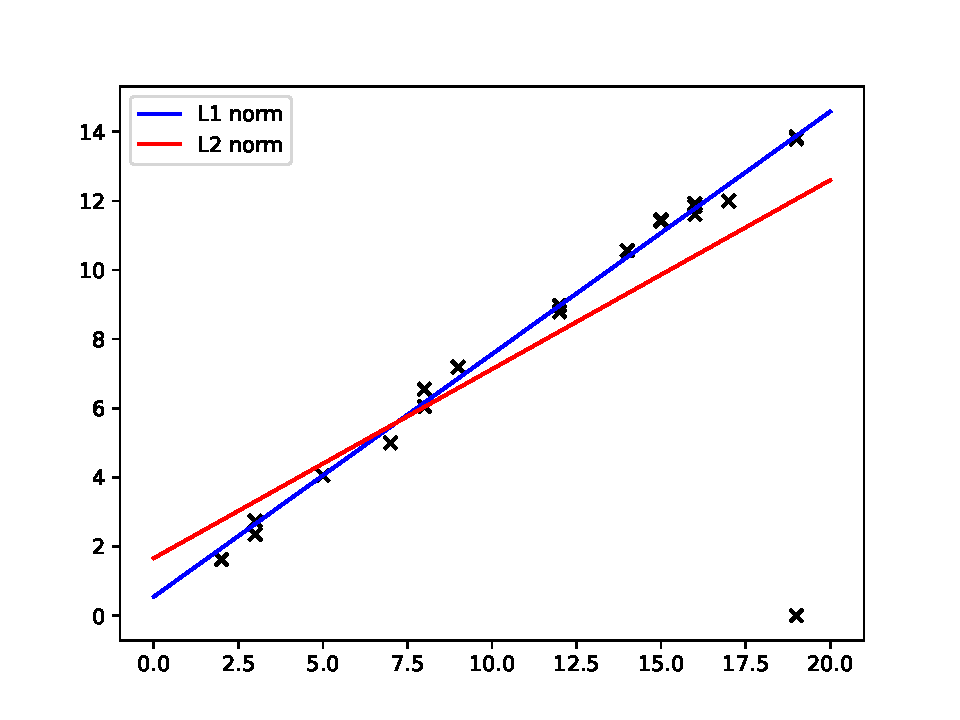
\includegraphics[width=7cm]{pics/chapter2/l1-l2-diff2.pdf}
    \end{minipage}
    \begin{minipage}[t]{0.48\textwidth}
    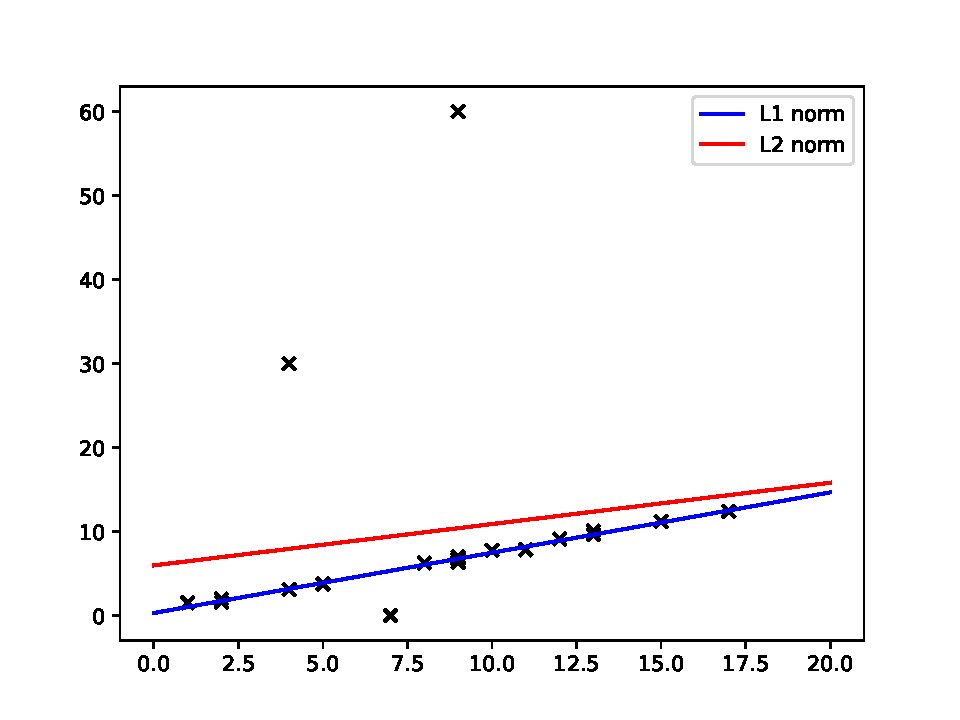
\includegraphics[width=7cm]{pics/chapter2/l1-l2-diff.pdf}
    \end{minipage}
    \caption{\small 数据含有离群值时最小二乘和最小绝对值回归的拟合情况}
    \label{fig2.1}

\end{figure}

我们使用$L_1$目标函数来估计$\bm{\beta}$,则其中$\bm{\beta}^*$为最小绝对值回归系数,$e$为一随机噪声,
可以写出最小绝对值回归的一般形式
\begin{equation} \label{l1losstotal}
    \begin{split}
    Y &= \bm{X}^T\bm{\beta}^* + e\\
    \bm{\beta}^* &= \underset{\bm{\beta}\in \mathbb{R}^{p}}{\operatorname {arg\ min}}
    \mathbb{E}|Y - X\bm{\beta}|.
    \end{split}
\end{equation}

\subsubsection{最小绝对值回归的估计方法}
对于\eqref{l1loss},它是一个凸优化问题,但是其不具备显式解,一般求它的数值解。但是其目标函数在$\bm{0}$点不可导,
因此不能直接使用使用梯度下降法,一般来说,该问题
的全局最优解可以通过求解下面的线性规划问题得到:
$$
    \underset{\bm{\beta}, \bm{t}}{\operatorname{min\ }} 1^T \bm{t}
$$
$$
    s.t. -\bm{t} \leq \bm{X}_{n\times p}\bm{\beta}_{p\times1} - \bm{Y}_{n\times 1} \leq \bm{t}
$$
目前对于线性规划问题已经有了比较成熟的解决方法,主要通过单纯形法或者内点法求解,后者的时间复杂度可以控制在多项式时间,
然而,一般而言,当$n$和$p$均很大时,上述线性规划问题面临很高的变量和约束维数,计算速度仍较慢。

由于$L_1$范数的目标函数在机器学习领域的大量使用,已经产生了一些光滑化方法,做法是用一个接近$L_1$的目标函数来替代它,
用来替代的函数往往处处可导,因而可以使用梯度下降法求解。
典型的代表就是使用Huber’s M统计量近似$L_1$范数目标函数\cite{lucas1997robustness},
\begin{equation*}
    \rho(e) = \left\{
        \begin{array}{clr}
            \frac1{2}e^2,\ |e| \leq \gamma \\
            \gamma |e| - \frac1{2}\gamma ^2 ,\ |e| > \gamma
        \end{array}
    \right.
\end{equation*}
其中$\gamma$为某一正数,该问题可以转化为一个二次规划问题求解。

\subsection{聚类——迭代拆解算法}
近年来针对最小绝对值回归的性能研究发展出了除了光滑化目标函数之外的方法,可以在不改变目标函数的情况下,
通过寻求新的优化方法进行求解。这样一来,可不改变最小绝对值回归估计量的统计性质。
这里介绍Park et al.(2019)提出的一种基于聚类——迭代拆解算法的最小绝对值回归求解方法\cite{park2021optimization}。

\subsubsection{聚类——迭代拆解算法说明}
聚类是一种在机器学习中常见的做法,就是按照某种给定的规则,将特征接近的样本点归类到一起。
聚类——迭代拆解算法的提出受到以下事实的启发:
1)优化问题面临的数据集规模庞大,其中许多的样本点在进行参数估计时的贡献很接近;
2)如果对相似的样本点进行聚类,提炼该聚类中的信息,避免每个样本点都进入计算,那么就会大大减小问题的规模;
3)假设在聚类后构造的新数据集上不能接近问题的最优解,那么就拆解当前的聚类,在新聚类上进行计算,
聚类个数有限,因此最坏情况下相当于直接求解原问题;

采用聚类——迭代拆解算法求解某个优化问题的前提如下:1)必须能够提出一种规则来对样本点聚类;
2)必须找到合适的聚类和拆解聚类的标准;
3)需要在聚类后构造的新数据集上明确定义新的优化问题;
4)能够判定当前解是否接近最优解。

\subsubsection{优化最小绝对值回归}
算法3.1给出了任何一个聚类——迭代拆解算法的主要步骤,注意算法3.1必然在某处停止,
因为每次不断拆解聚类,当聚类个数$|K^{t}|= n$时,相当于计算原问题,此时算法终止。
\begin{table}[H]%%%%%%开始表格
    \centering%把表居中
    \begin{tabular}{{p{0.9\columnwidth}}}%三个c代表该表一共三列,内容全部居中
    
    \toprule%第一道横线 表头
    {\heiti 算法} {\bf3.1} 聚类——迭代拆解算法(Aggregate and Iterative Disaggregate, AID) \\
    \midrule%第二道横线 符号+解释+单位 中间用&隔开
    输入:原始数据集$\bm{X}_{n\times p}$,样本点的下标集合${I} = \{1, 2, ..., n\}$,
    数据的特征下标集合${J} = {1, 2, ..., p}$,原优化问题$P$。\\
    初始化:对原始数据集$\bm{X}$聚类,然后按某种规则产生新的优化数据集$\bm{X}^{(1)}$。 \\
    对于$t = 1, ..., \tau$:\\
        记${C}^{(t)} = \{{C}_1^{(t)}, ..., C_K^{(t)}\}$为聚类的集合, $K^{(t)} = \{1, ..., |K^{(t)}|\}$为当前聚类的下标,
        \\
        1.根据当前聚类情况${C}^{(t)}$,构造新的数据集$\bm{X}^{(t)}$,求解相应的优化问题${P}^{(t)}$; \\
        2.检查解$\bm{s}^{(t)}$是否达到最优条件;\\
        3.如果不满足条件,拆解当前聚类。
        \\
    \bottomrule%第三道横线
    \end{tabular}
\end{table}%%%%%%结束表格

改写\eqref{l1loss}的目标函数,
\begin{equation}\label{l1loss2}
\xi^* = \underset{\bm{\beta} \in \mathbb{R}^{p}}{\operatorname{min}} 
\sum_{i \in I}|y_i - \sum_{j \in J}x_{ij}\bm{\beta}_j|
\end{equation}

首先给出聚类方法。给定$|K^{(0)}|$为目标聚类个数,初始化$C^{(0)} = \{C_1^{(0)}, C_2^{(0)}, ..., C_K^{(0)}\}$,
我们可以使用任意的聚类方法进行初始化。接下来给出如何根据聚类来产生新的数据集,
对于在任一迭代周期内产生的聚类$C^{(t)}_k, k = 1, ..., K^{(t)}$,取
\begin{equation*}
    x_{kj}^{(t)} = \frac{\sum_{i \in C_k^{(t)}}x_{ij}}{|C_k^{(t)}|},\ j \in J \  
    \text{并且} \
    y_{k}^{(t)} = \frac{\sum_{i \in C_k^{(t)}}y_i}{|C_k^{(t)}|}
\end{equation*}

对于每一个不同的聚类需要给出一个权重来区分信息量不同的聚类,因此在新的数据集上,我们求解下面的问题
\begin{equation}\label{clusterl1}
    F^{(t)} =\underset{\bm{\beta}^{(t)} \in \mathbb{R}^{p}}{\operatorname{min}} 
    \sum_{k=1}^{K^{(t)}}|C_k^{(t)}||y_k^{(t)} - \sum_{j \in J}x_{kj}^{(t)}\bm{\beta}_j^{(t)}|
\end{equation}
容易发现,任何\eqref{clusterl1}的可行解都是\eqref{l1loss2}的可行解。
记$\hat{\bm{\beta}}^{(t)}$为\eqref{clusterl1}的解,在每次迭代,我们计算此时的原目标函数的取值
\begin{equation}
    \xi^{(t)} = \sum_{i \in I} |y_i - \sum_{j \in J}x_{ij}\hat{\bm{\beta}}_j^{(t)}|
\end{equation}

接下来给出拆解聚类的准则:设$t$步的聚类集合为$C^{(t)}$,该步解为$\hat{\bm{\beta}}^{(t)}$,
对于$k = 1, ..., K^{(t)}$,计算$\theta_i = y_i - \sum_{j \in J}x_{ij}\hat{\bm{\beta}}_j^{(t)}$,

1)若对于任意$i \in C_k^{(t)}$,$\theta_i$有相同的符号,那么该聚类$C^{(t)}_k$将保留到下次迭代,即$C^{(t+1)} \leftarrow C^{(t+1)}\bigcup C^{(t)}_k$,见图
\ref{aid-demo};

2)若不满足上述条件,那么根据$\theta_i$符号异同,将$C^{(t)}_k$分成两个集合,$C_{k+}^{(t)} = \{i \in C_k^{(t)} | \theta_i > 0\}$ ,
$C_{k-}^{(t)} = \{i \in C_k^{(t)} | \theta_i < 0\}$,见图\ref{aid-demo}b,这两个集合在下一步形成新的聚类,
即$C^{(t+1)} \leftarrow C^{(t+1)}\bigcup \{ C_{k+}^{(t)}, C_{k-}^{(t)}\}$,见图\ref{aid-demo}c。

\begin{figure}[H]
    \centering
    \begin{subfigure}[t]{0.3\textwidth}\label{aid-demo1}
    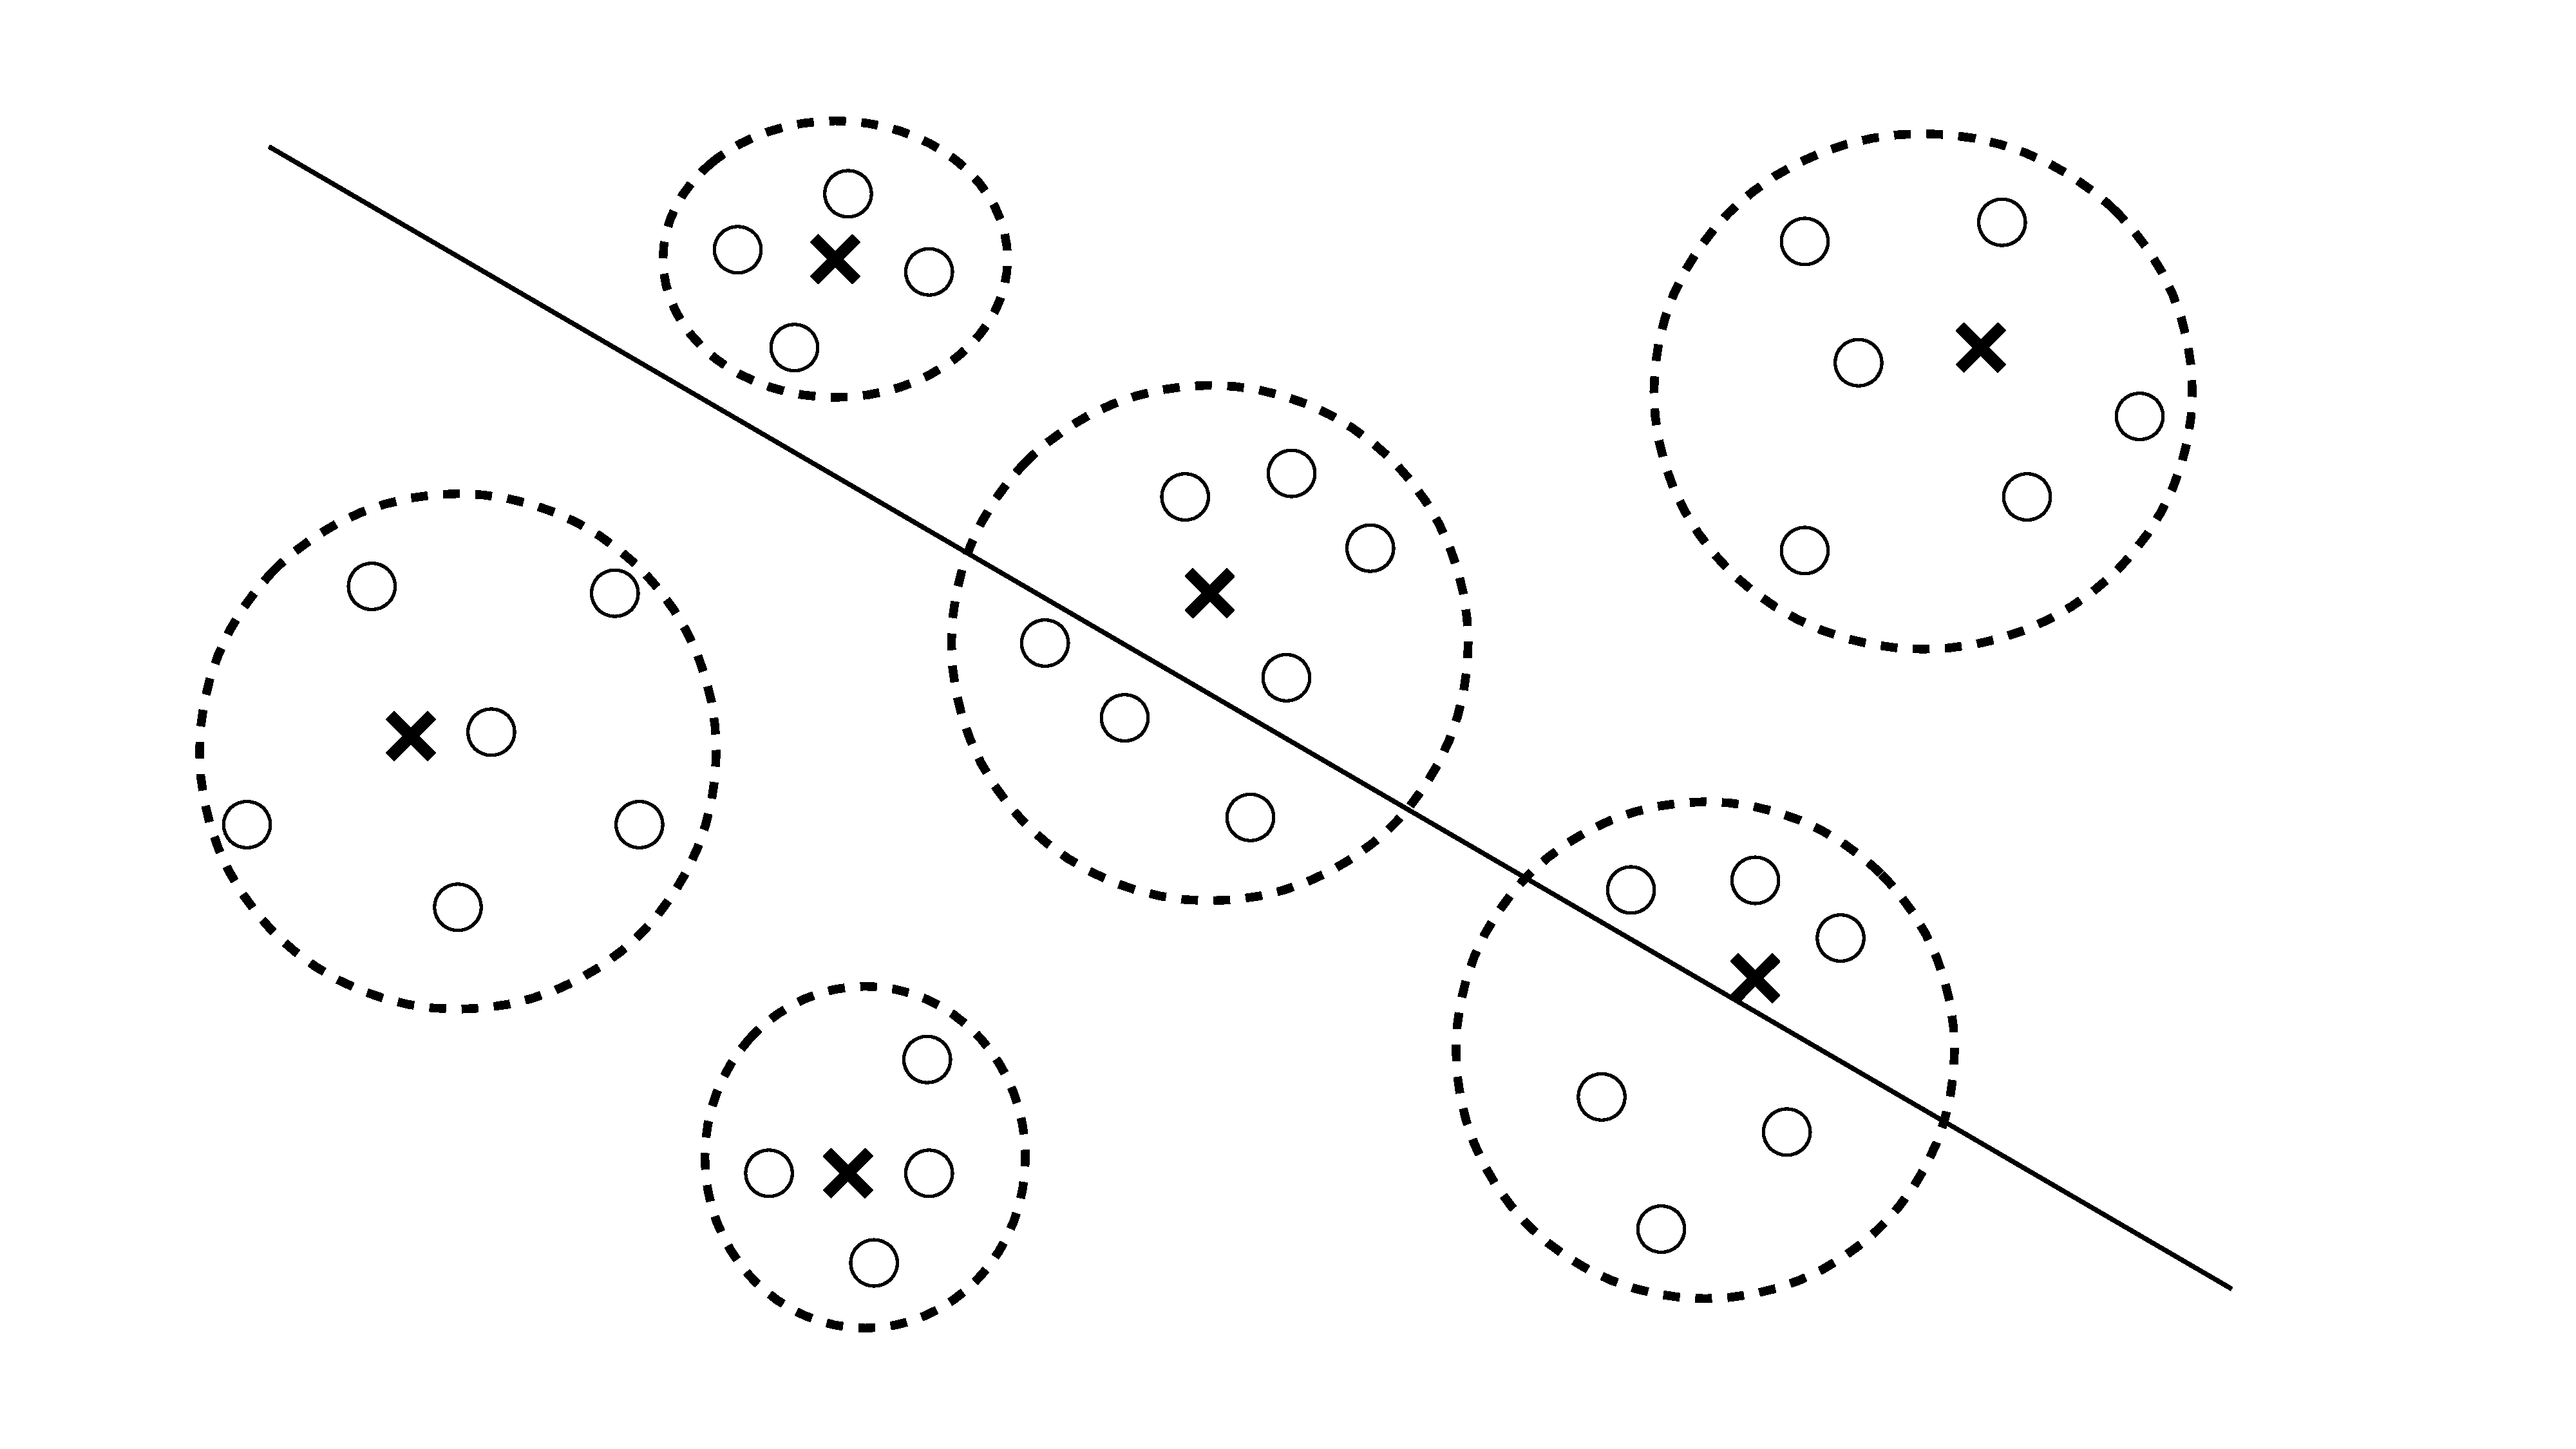
\includegraphics[width=4.9cm]{pics/chapter2/aid-demo-a.pdf}
    \captionof{figure}{}
    \end{subfigure}
    \begin{subfigure}[t]{0.3\textwidth}\label{aid-demo2}
    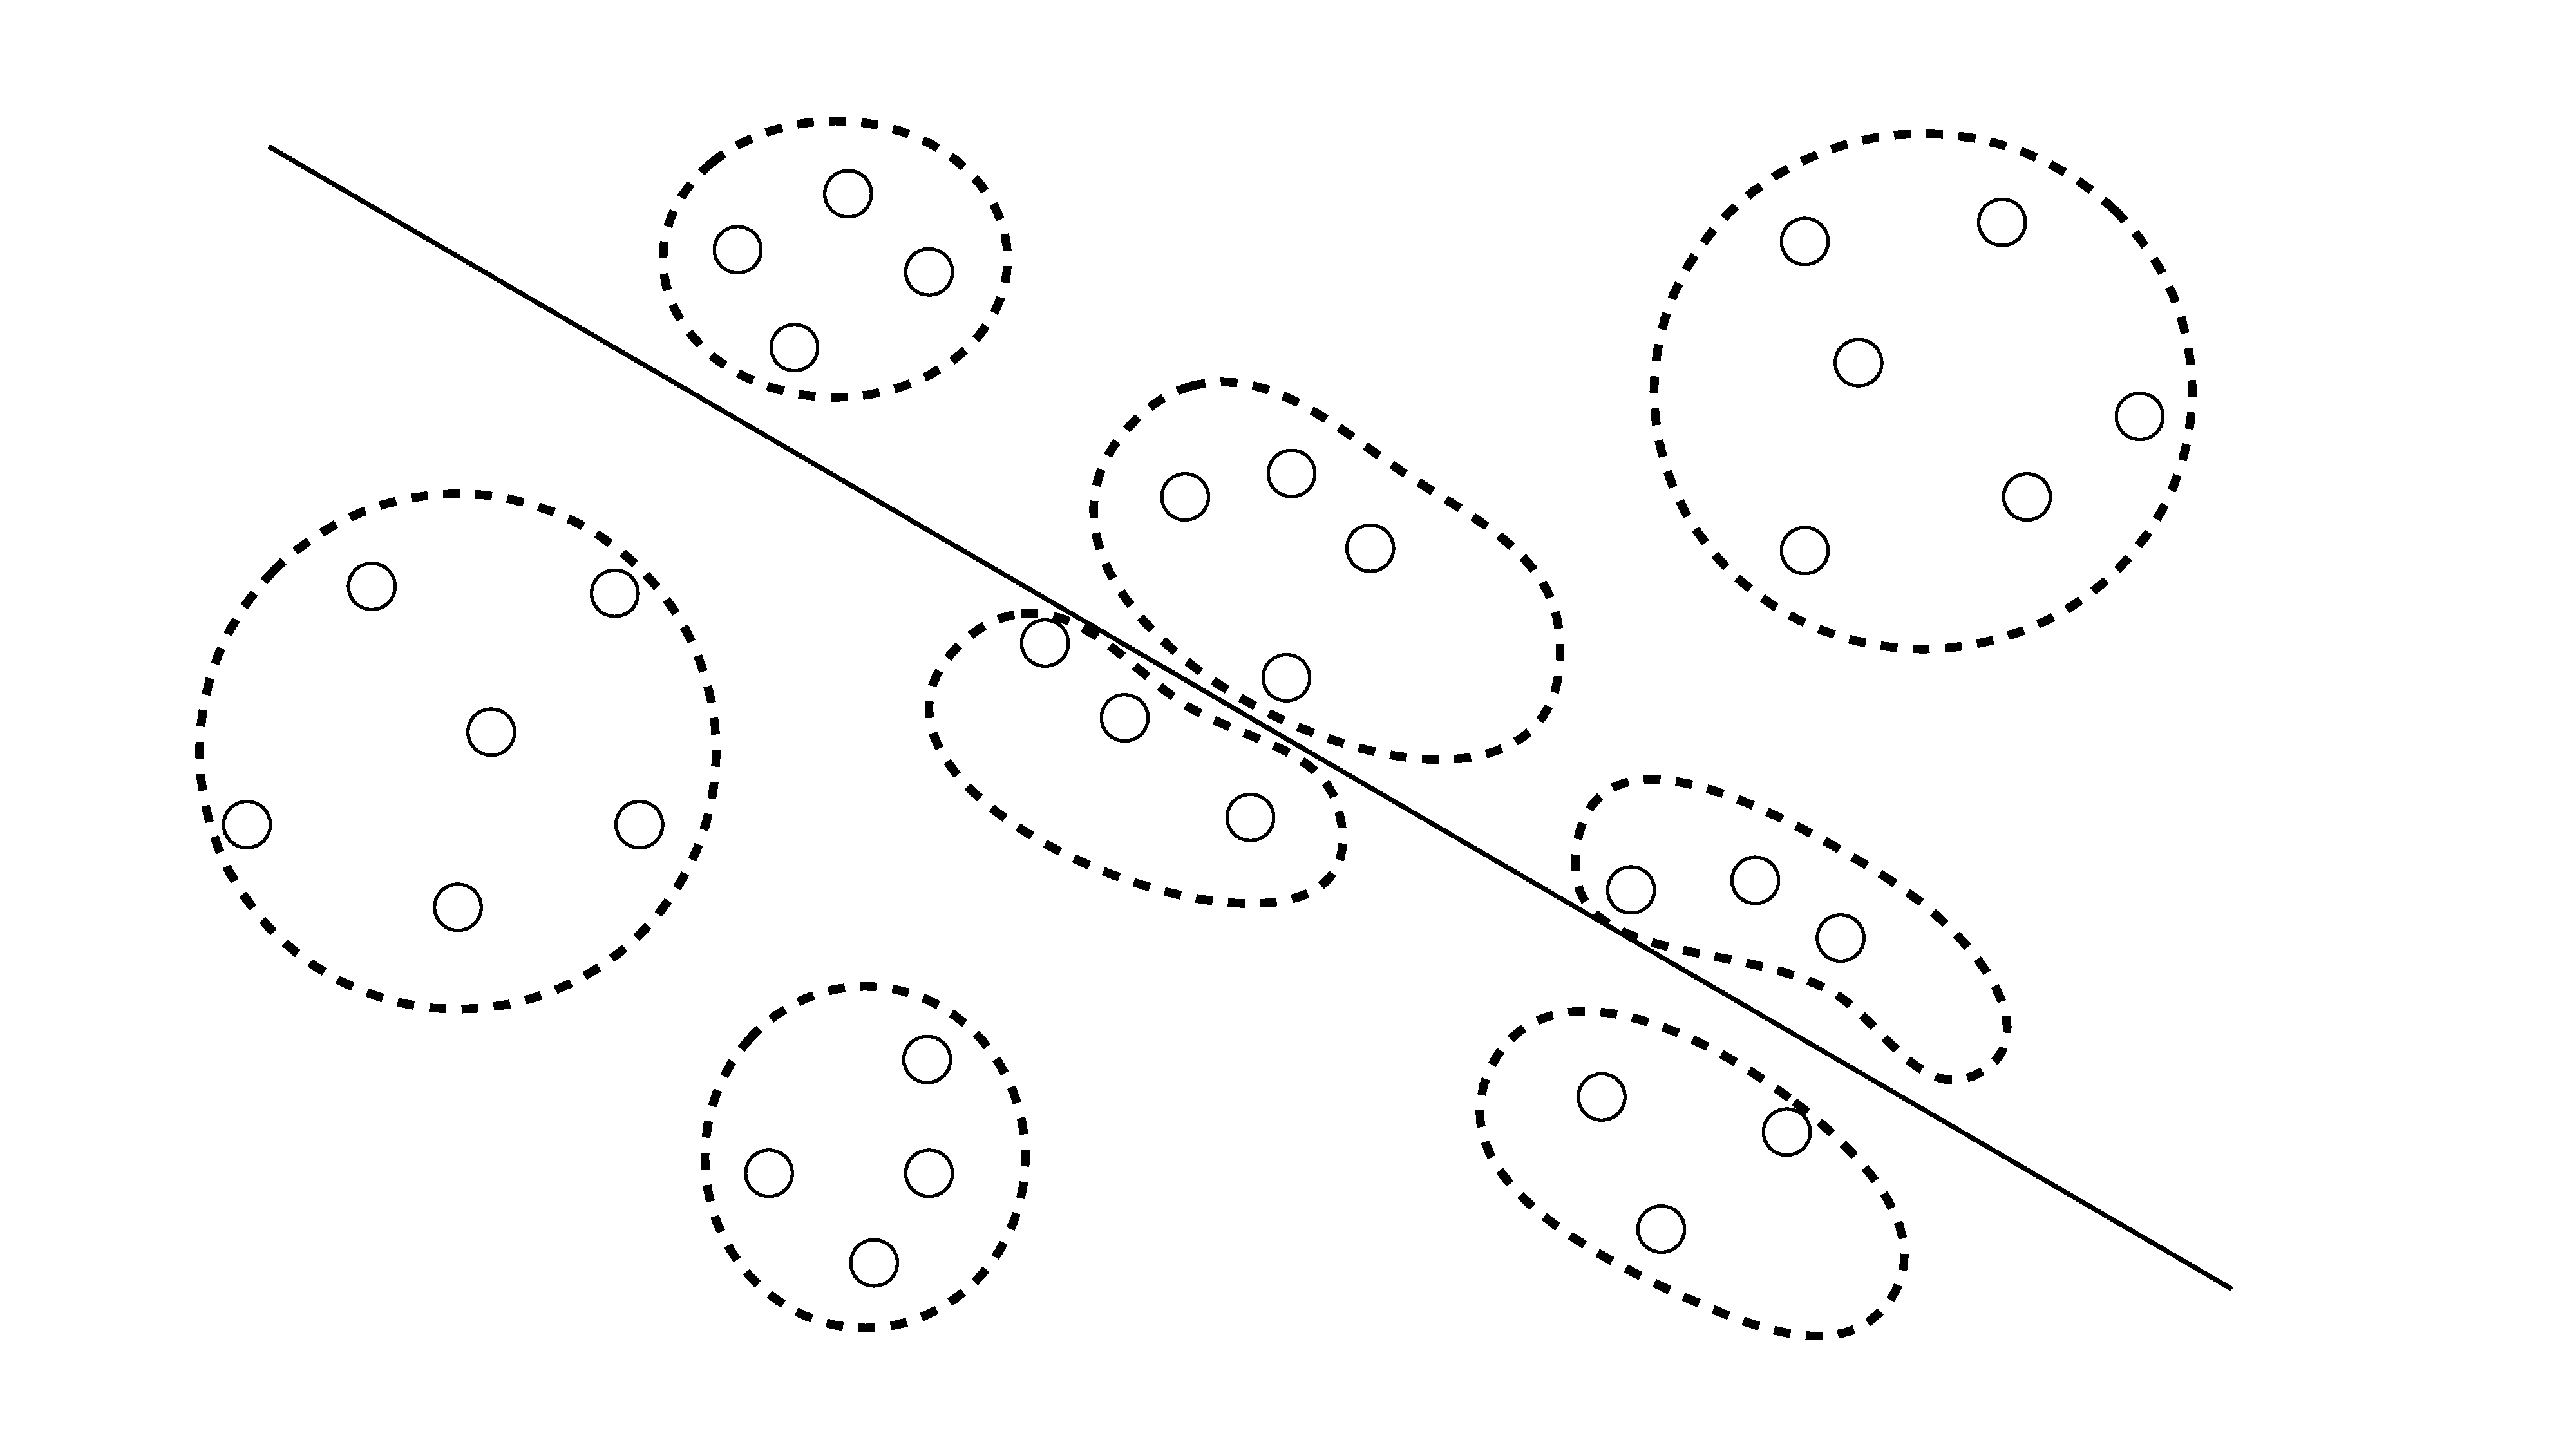
\includegraphics[width=4.9cm]{pics/chapter2/aid-demo-b.pdf}
    \captionof{figure}{}
    \end{subfigure}
    \begin{subfigure}[t]{0.3\textwidth}\label{aid-demo3}
    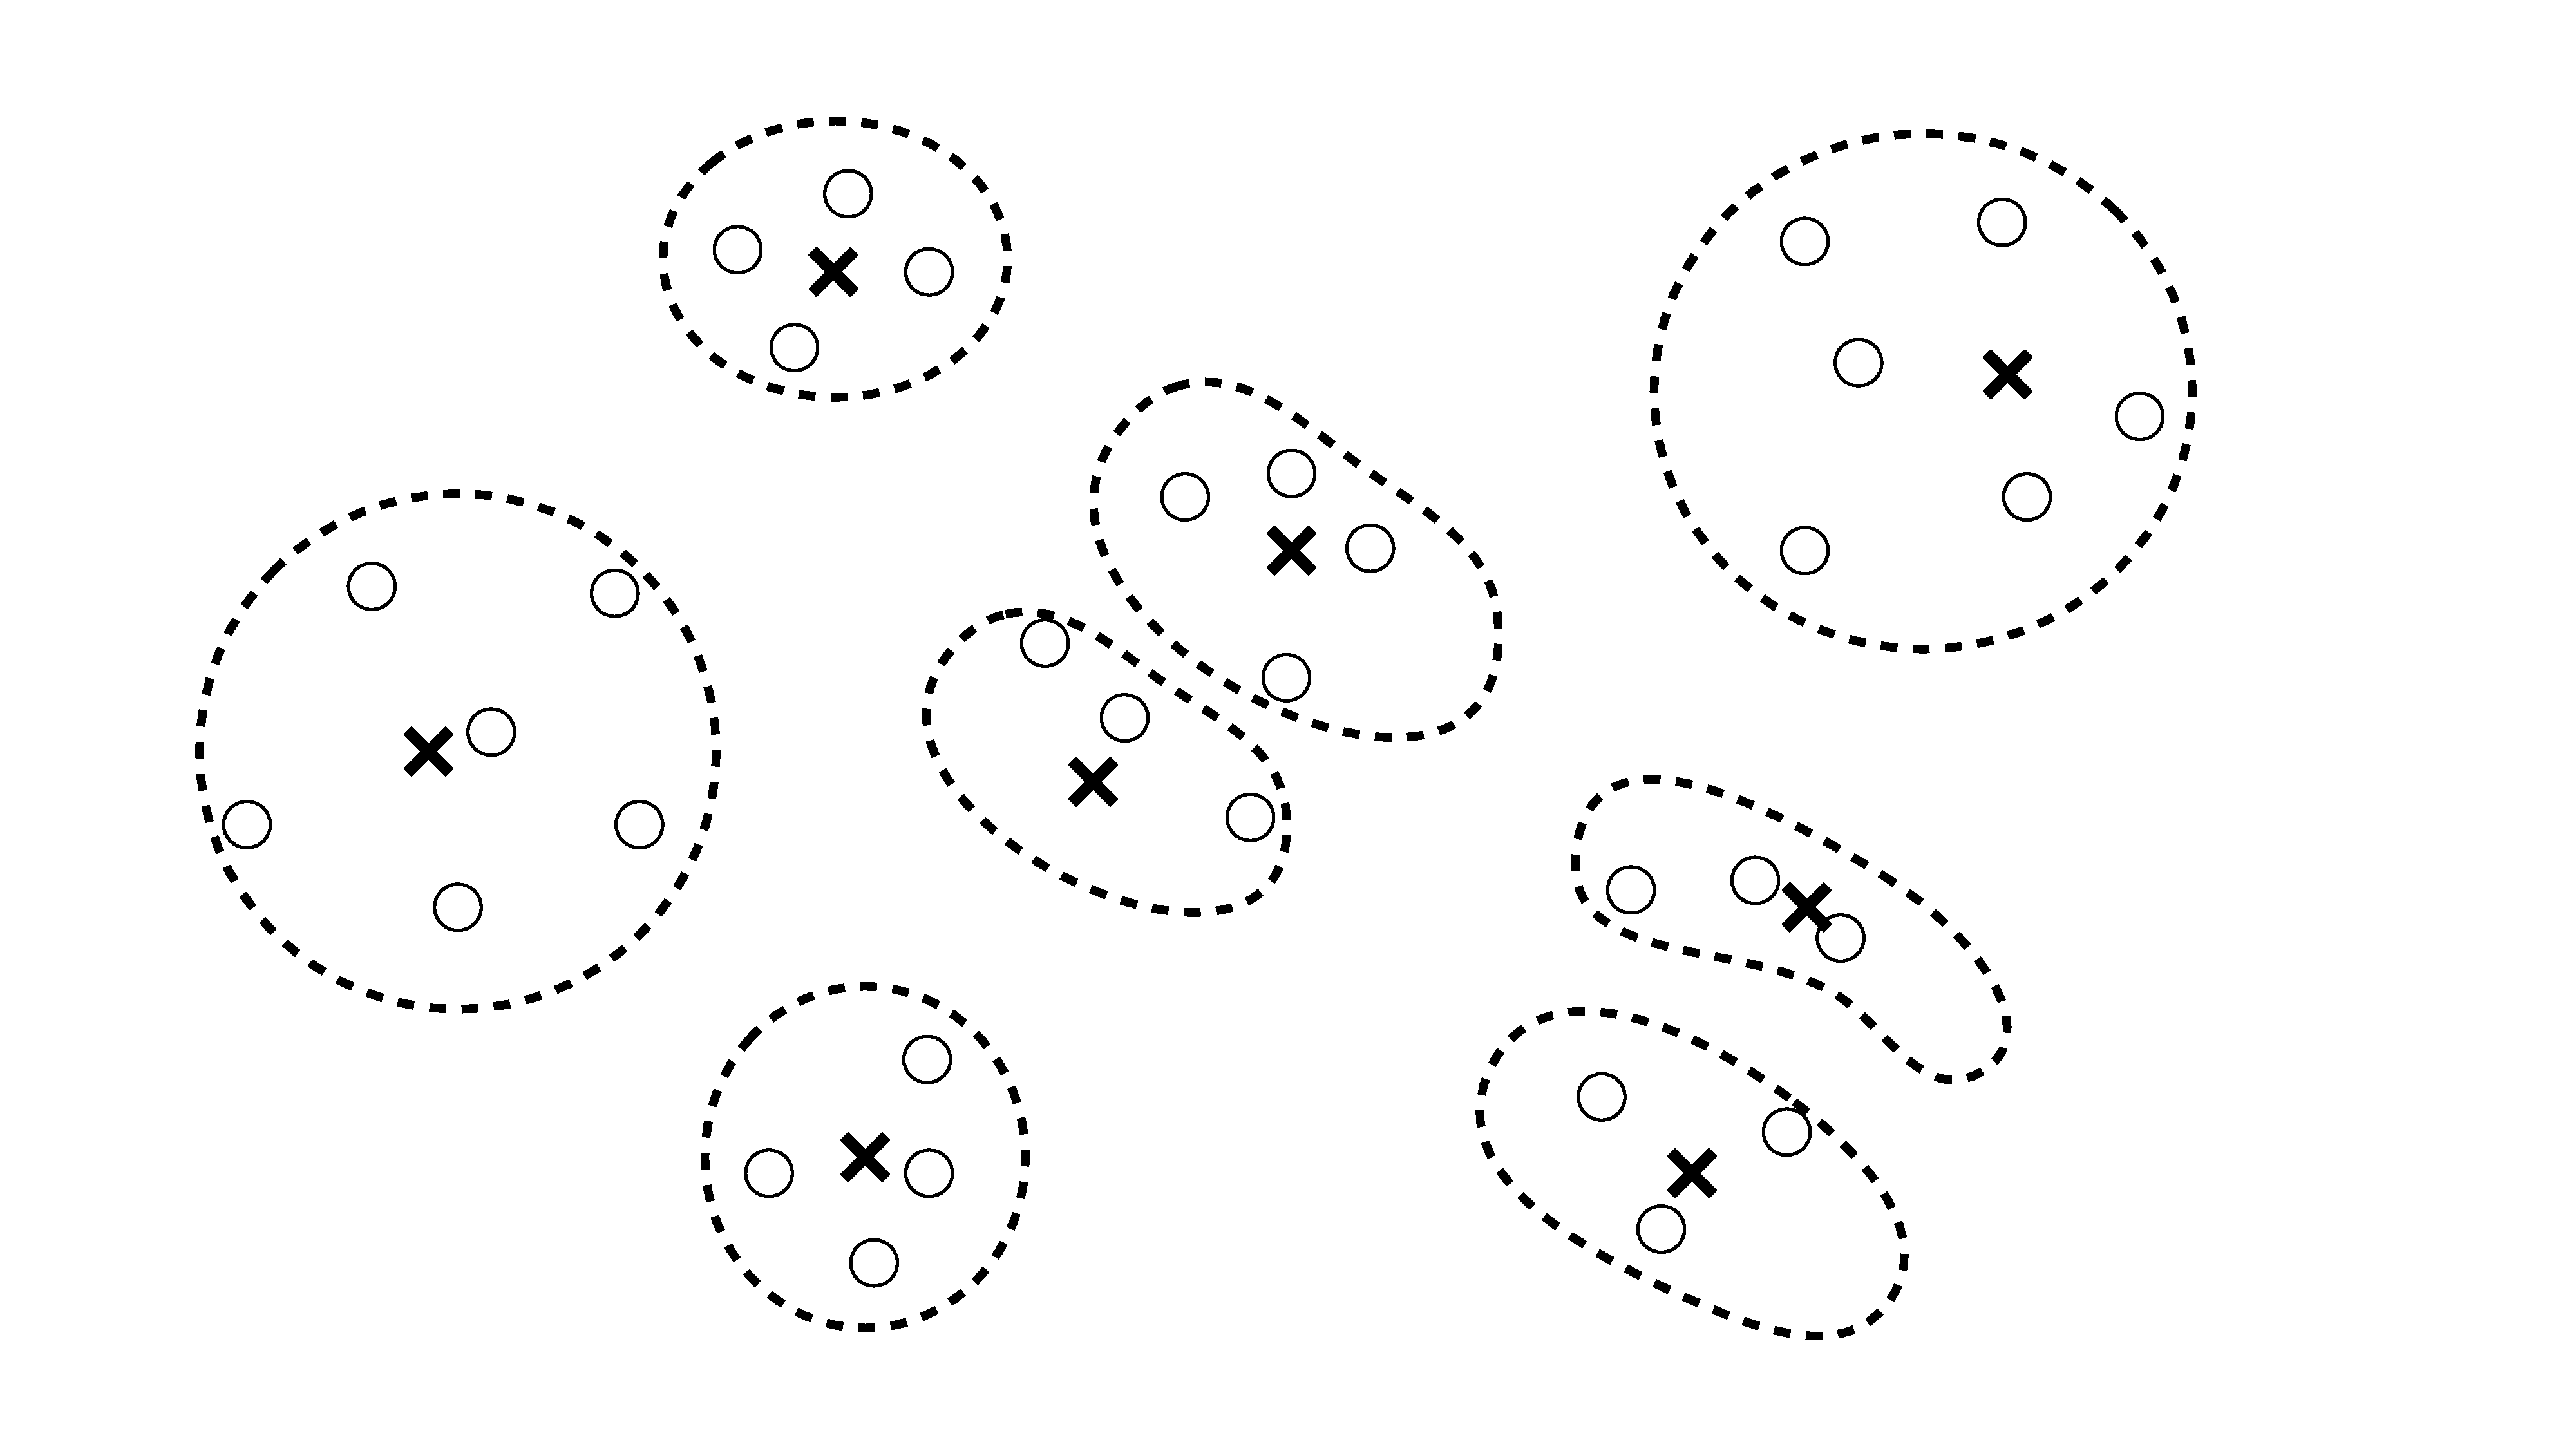
\includegraphics[width=4.9cm]{pics/chapter2/aid-demo-c.pdf}
    \captionof{figure}{}
    \end{subfigure}
    \caption{\small 聚类拆解步骤示意图}
    \label{aid-demo}

\end{figure}

结合算法3.1,到这里已经给出了完成聚类——迭代拆解最小绝对值回归的所有计算步骤,当聚类无法继续划分时,迭代终止。

下面证明最后一次迭代的解$\hat{\bm{\beta}}^{(\tau)}$就是\eqref{l1loss2}的解$\bm{\beta}^*$,
\begin{equation*}
    \begin{split}
        \xi^* & = \sum_{i \in I} |y_i - \sum_{j \in J}x_{ij}\bm{\beta}_j^*|
        = \sum_{k \in K^{(t)}}\sum_{i \in C_k^{(t)}}|y_i - \sum_{j \in J}x_{ij}\bm{\beta}_j^*| \\
        & \geq \sum_{k \in K^{(t)}}|\sum_{i\in C_k^{(t)}}(y_i - \sum_{j \in J}x_{ij}\bm{\beta}_j^*)|
        = \sum_{k \in K^{(t)}}|C_k^{(t)}||y_k^{(t)} - \sum_{j \in J}x_{kj}^{(t)}\bm{\beta}_j^*|\\
        & \geq \sum_{k \in K^{(t)}} |C_k^{(t)}||y_K^{(t)} - \sum_{j\in J}x_{kj}^{(t)} \hat{\bm{\beta}}_j^{(t)}|
        = \sum_{k \in K^{(t)}} |\sum_{i \in C_k^{(t)}} y_i - \sum_{i \in C_k^{(t)}}\sum_{j \in J}x_{ij}\hat{\bm{\beta}}_j^{(t)}| \\
        & = \sum_{k \in K^{(t)}} \sum_{i \in C_k^{(t)}}|y_i - \sum_{j \in J}x_{ij}\hat{\bm{\beta}}_j^{(t)}|
        = \sum_{i \in I}|y_i - \sum_{j \in J} x_{ij} \hat{\bm{\beta}}_j^{(t)}| 
        = \xi^{(t)}
    \end{split}
\end{equation*}

因为$\hat{\bm{\beta}}_j^{(t)}$是\eqref{l1loss2}的可行解,又显然$\xi^* \leq \xi^{(t)}$,
这就证明了$\xi^* = \xi^{(t)}$,注意到$ \sum_{k \in K^{(t)}} |C_k^{(t)}||y_K^{(t)} - \sum_{j\in J}x_{kj} \hat{\bm{\beta}}_j^{(t)}|$
就是$F^{(t)}$,因此$\xi^{(t)} = F^{(t)}$。因此最后一次迭代$F^{(\tau)}$的最优解$\hat{\bm{\beta}}^{(\tau)}$就是原问题的最优解。

\subsubsection{优化带有惩罚项的最小绝对值回归}
前面给出的算法已经在很大程度上优化了在处理高维宏观经济变量时,最小绝对值回归计算性能的问题。
而在高维宏观经济实证研究中,变量的维数众多,在建立最小绝对值回归模型时,还需要考虑到变量筛选问题。

对于\eqref{l1losstotal},为了进行变量的筛选,我们需要对估计量$\bm{\beta}^*$的维数做出约束,
一般来说,我们通常采用以下3三种方法:1)$\|\bm{\beta}\|_0 = p$,可以直接选择入选变量的个数;
2)$\|\bm{\beta}\|_2 < s$,该法又称为岭回归;3)$\|\bm{\beta}\|_1 < s$,即为常用的$L_1$正则化方法。
通过加入新的约束,问题的形式也发生了变化。

Park et al.(2021)给出了进一步的结论\cite{park2021optimization},对于问题
\begin{equation}\label{l1conclusion}
    E^* = \underset{B\in \phi}{\operatorname{min}} ||Y - f(X, B)||_{L_1}
\end{equation}
其中$Y$为模型响应变量数据矩阵,$X$为解释变量数据矩阵,$B$为模型系数矩阵,$\phi$为模型系数的约束条件。
$f$为任一目标函数,若$f$满足条件
\begin{equation}\label{fcondition}
    f(B, WX) = Wf(B, X)
\end{equation}
其中$W$为一权重矩阵。那么就可以通过聚类——迭代拆解算法求原优化问题的最优解。

而在岭回归和LASSO中,都通过给目标函数加上惩罚项来进行求解,岭回归对应的惩罚项$s\sum_{i=1}^p\bm{\beta}_i^2$,
$L_1$正则化对应的惩罚项为$s\sum_{i=1}^p|\bm{\beta}_i|$,容易发现,加入惩罚项后目标函数仍然满足\eqref{fcondition}
。因此,对于需要进行变量筛选的高维最小绝对值回归问题,我们可以修改目标函数,通过算法3.1解决。
对于携带正则项的最小绝对值回归,也可以通过线性规划来处理\cite{wang2006regularized}。

\subsection{一种基于替代变量的估计方法}
聚类——迭代拆解算法是通过有效减少$L_1$目标函数最小化的问题规模来提升求解性能,
每一次迭代仍需要通过线性规划方法求解$L_1$目标函数的最小化问题。
luciani2014large et al.(2020)提出了一种基于替代变量的估计方法\cite{svn},通过替代变量将分位数损失函数转化为$L_2$损失函数,
避免使用线性规划求解分位数损失,因此可以显著提升一般分位数回归的求解性能。

考虑到最小绝对值回归为其特殊情形,因此该算法可以在一定程度上解决最小绝对值回归的性能问题。
下面我们介绍如何将该方法应用在最小绝对值回归的场景下,并且给出具体的计算步骤。

\subsubsection{基于替代变量的迭代算法}
考虑\eqref{l1losstotal},
对目标函数稍作形式变换,其中$\rho(x) = x(0.5 - \mathbb{I}[x \leq 0])$,
$\mathbb{I}(x)$为指示函数。
\begin{equation}
\bm{\beta}^* = \underset{\bm{\beta} \in \mathbb{R}^{p}}{\operatorname{arg\ min}}\mathbb{E}|Y - \bm{X}^T\bm{\beta}| = 
\underset{\bm{\beta} \in \mathbb{R}^{p}}{\operatorname{arg\ min}}\mathbb{E}\rho(Y - \bm{X}^T\bm{\beta})
\end{equation}
若已知n\ $i.i.d.$ 的样本$(\bm{X}_i, Y_i)\ (1 \leq i \leq n)$,令$\hat{\bm{\beta}}$为$\bm{\beta}^*$的估计量,
\begin{equation}\label{rho-problem}
    \hat{\bm{\beta}} = \underset{\bm{\beta} \in \mathbb{R}^{p}}{\operatorname{arg\ min}}\frac1{n}\sum_{i=1}^{n}\rho(Y_i - \bm{X}_i^T\bm{\beta}).
\end{equation}

一般地,我们使用牛顿迭代法求解某随机优化问题:
\begin{equation}\label{randomversion}
    \bm{\beta}^* = \underset{\bm{\beta} \in \mathbb{R}^{p}}{\operatorname{arg\ min}} \mathbb{E}[G(\bm{\beta};\bm{X},Y)]
\end{equation}
其中$G(\bm{\beta};\bm{X}, Y)$是损失函数,$\bm{X}$和$Y$分别是$p$维自变量和一元响应变量,$\bm{\beta}$为回归系数。使用牛顿-拉弗森迭代来求解,
\begin{equation}
    \tilde{\bm{\beta}}_1 = \bm{\beta}_0 - \bm{H}(\bm{\beta}_0)^{-1}\mathbb{E}[g(\bm{\beta};\bm{X},Y)]
\end{equation}
其中$\bm{\beta}_0$是一个初始估计,$g(\bm{\beta};\bm{X},Y)$为损失函数$G(\bm{\beta};\bm{X},Y)$关于$\bm{\beta}$的梯度。\\
$\bm{H}(\bm{\beta}):=\partial\mathbb{E}[g(\bm{\beta};\bm{X},Y)
/\partial\bm{\beta}$表示$\mathbb{E}G(\bm{\beta};\bm{X},Y)$的海森矩阵(Hessian Matrix)。特别地,我们这里考虑损失函数为$L_1$损失的特殊情形,
\begin{equation}\label{rho-condition}
    G(\bm{\beta};\bm{X},Y) = \rho(Y - \bm{X}^T\bm{\beta})
\end{equation}
在\eqref{rho-condition}的情形下,$g(\bm{\beta};\bm{X},Y) = \bm{X}(\mathbb{I}[Y - \bm{X}^T\bm{\beta} < 0] - 0.5)$。

并且$\bm{H}(\bm{\beta}) = \mathbb{E}(\bm{X}\bm{X}^Tf(\bm{X}^T(\bm{\beta} - \bm{\beta}^*)))$,这里
$f(x)$是噪声$e$的密度函数。当初始估计量$\bm{\beta}_0$和$\bm{\beta}^*$很接近时,$\bm{H}(\bm{\beta}_0)$就会很接近
$\bm{H}(\bm{\beta}^*) = \bm{\Sigma}f(0)$,这里$\bm{\Sigma} = \mathbb{E}\bm{X}\bm{X}^T$是$\bm{X}$的协方差
矩阵。使用$\bm{H}(\bm{\beta}^*)$替换$\bm{H}(\bm{\beta}_0)$,可得
\begin{equation}\label{rho-beta1}
    \bm{\beta}_1 = \bm{\beta}_0 - \bm{H}(\bm{\beta}^*)^{-1}\mathbb{E}[g(\bm{\beta};\bm{X}, Y)]
    = \bm{\beta}_0 - \bm{\Sigma}^{-1}f^{-1}(0)\mathbb{E}[g(\bm{\beta}_0;\bm{X},Y)]
\end{equation}
在$\bm{\beta}^*$处对$\mathbb{E}[g(\bm{\beta}_0;\bm{X},Y)$进行泰勒展开,
\begin{equation*}
    \begin{split}
\mathbb{E}[g(\bm{\beta}_0;\bm{X},Y) &= \bm{H}(\bm{\beta}^*)(\bm{\beta}_0 - \bm{\beta}^*) + O(|\bm{\beta}_0 - \bm{\beta}^*|_2^2) \\
 &= \bm{\Sigma}f(0)(\bm{\beta}_0 - \bm{\beta}^*) + O(|\bm{\beta}_0 - \bm{\beta}^*|_2^2)
    \end{split}
\end{equation*}
结合\eqref{rho-beta1},可以得到
\begin{equation*}
    \begin{split}
        |\bm{\beta}_1 - \bm{\beta}^*|_2 &=  |\bm{\beta}_0 - \bm{\Sigma}^{-1}f^{-1}(0)(
            \bm{\Sigma}f(0)(\bm{\beta}_0 - \bm{\beta}^*) + O(|\bm{\beta}_0 - \bm{\beta}^*|_2^2)
        ) - \bm{\beta}^*|_2\\
        &= O(|\bm{\beta}_0 - \bm{\beta}^*|_2^2)
    \end{split}
\end{equation*}
因此,如果我们得到一个$\bm{\beta}^*$的一致估计量$\bm{\beta}_0$,我们就可以通过\eqref{rho-beta1}得到
偏误更小的估计。

下面我们将\eqref{rho-beta1}转化成一个最小二乘问题。首先我们重写该式,
\begin{equation}
    \begin{split}
    \bm{\beta}_1 &= \bm{\Sigma}^{-1}(\bm{\Sigma}\bm{\beta}_0 - f^{-1}(0)\mathbb{E}[g(\bm{\beta}_0;\bm{X},Y)])\\
    &= \bm{\Sigma}^{-1}\mathbb{E}[\bm{X}\{\bm{X}^T\bm{\beta}_0 - f^{-1}(0)(\mathbb{I}[Y \leq \bm{X}^T\bm{\beta}_0] - 0.5)\}]
    \end{split}
\end{equation}
这里我们定义一个新的响应变量$\tilde Y$,
\begin{equation}
    \tilde Y = \bm{X}^T\bm{\beta}_0 - f^{-1}(0) (\mathbb{I}[Y \leq \bm{X}^T\bm{\beta}_0] - 0.5)
\end{equation}
那么$\bm{\beta}_1 = \bm{\Sigma}^{-1}\mathbb{E}(\bm{X}\tilde{Y})$就是线性回归问题$\tilde Y = \bm{X}^T\bm{\beta}$
的最优回归系数,即
\begin{equation}\label{beta1-original}
    \bm{\beta}_1 = \underset{\bm{\beta} \in \mathbb{R}^{p}}{\operatorname{arg\ min}} 
    \mathbb{E}(\tilde Y - \bm{X}^T \bm{\beta})^2
\end{equation}
给定$i.i.d.$样本$(\bm{X}_i, Y_i)$,构造
\begin{equation}\label{svny}
    \tilde{Y}_i = \bm{X}_i^T\hat{\bm{\beta}}_0 - \hat{f}^{-1}(0)
    (\mathbb{I}[Y_i \leq \bm{X}_i^T \hat{\bm{\beta}}_0] - 0.5)
\end{equation}
其中$\hat{\bm{\beta}}_0$为$\bm{\beta}^*$的一个初始估计,$\hat{f}(0)$为$f(0)$的一个估计
\begin{equation}\label{yl2loss}
    \hat{\bm{\beta}} = \underset{\bm{\beta} \in \mathbb{R}^{p}}{\operatorname{arg\ min}}
    \frac1{n} \sum_{i=1}^n(\tilde{Y}_i - \bm{X}_i^T\bm{\beta})^2
\end{equation}
这里我们选择某估计量作为$\hat{\bm{\beta}}_0$,并且采用$f(0)$的核密度估计作为$\hat{f}(0)$,

$$
    \hat{f}(0) = \frac1{nh}\sum_{i=1}^nK(\frac{Y_i - \bm{X}^T_i\hat{\bm{\beta}}_0}{h})
$$
其中$K(x)$为核函数,$h \rightarrow 0$是带宽,本方法
在每次迭代都需要调整带宽\cite{svn}。

只要给定的初始值$\hat{\bm{\beta}}_0$是$\bm{\beta}^*$的一致估计量,那么$\hat{\bm{\beta}}$就将会是一个更加接近
$\bm{\beta}^*$的新的估计,并且\eqref{yl2loss}为最小二乘问题,其计算十分简便。

我们当然可以将$\hat{\bm{\beta}}$作为\eqref{rho-beta1}的初始值,这样继续构造替代变量进行迭代,最终收敛到$\bm{\beta}^*$。
算法3.2给出了使用替代变量估计方法的计算步骤。
\begin{table}[H]%%%%%%开始表格
    \centering%把表居中
    \begin{tabular}{{p{0.9\columnwidth}}}%三个c代表该表一共三列,内容全部居中
    
    \toprule%第一道横线 表头
    {\heiti 算法}{\bf 3.2} 使用替代变量迭代算法方法求解最小绝对值回归问题(SVN, Substitue Variable Newton method)\\
    \midrule%第二道横线 符号+解释+单位 中间用&隔开
    输入:$Y$和$\bm{X}$的样本$\bm{Y} = (Y_1, Y_2, ..., Y_n)$,$\bm{X} = (\bm{X}^{\rm T}_1, \bm{X}^T_2, ..., \bm{X}^T_n)$,
    迭代次数$\tau$,核函数$K(x)$,依赖于迭代次数的带宽$h^{(t)}$,$(t = 1, ..., \tau)$。
    \\
    初始化:给出初始相合估计量$\hat{\bm{\beta}}^{0} $,将样本划分成$J$个均等子集,样本量均为$m$,为了给出最小绝对值回归估计量的相合估计,
    我们取任一子集里面的数据,直接使用最小一乘法估计$\hat{\bm{\beta}}^{0}$。
    \\
    对于$t = 1, ..., \tau$:
    取新的数据子集,在该数据集上
    \\
        1. 计算$\hat{f}^{(t)}(0)$,
        $$
        \hat{f}^{(t)}(0) = \frac1{mh}\sum_{i=1}^{m}K(\frac{Y_i - \bm{X}_i^T\hat{\bm{\beta}}^{(t-1)}}{h^{(t)}})
        $$
    \\
        2. 计算$\tilde{Y} = (\tilde Y_1, \tilde Y_2, ..., \tilde Y_m)$,
        $$
        \tilde{Y}_i = \bm{X}^T_i\hat{\bm{\beta}}^{(t-1)} - \hat{f}^{(t)}(0)^{-1}
        (\mathbb{I}[Y_i \leq \bm{X}_i^T \hat{\bm{\beta}}^{(t-1)}] - 0.5)
        $$
    \\
        3. 计算$\hat{\bm{\beta}}^{(t)}$,
        $$
        \hat{\bm{\beta}}^{(t)} = \underset{\bm{\beta} \in \mathbb{R}^{p}}{\operatorname{art\ min}}
        \frac1{m}\sum_{i=1}^m (\tilde{Y}_i - \bm{X}_i^T\bm{\beta})^2
        $$
    \\
    输出:$\hat{\bm{\beta}}^{(\tau)}$
    \\
    \bottomrule%第三道横线
    \end{tabular}
\end{table}%%%%%%结束表格

\subsubsection{优化带有惩罚项的最小绝对值回归}
在高维相依自变量的情形下,我们只需在\eqref{beta1-original}加入惩罚项即可,例如我们使用$L_1$正则化,那么
\begin{equation}
    \bm{\beta}_{1, \lambda} =\underset{\bm{\beta} \in \mathbb{R}^{p}}{\operatorname{arg\ min}} 
    \mathbb{E}(\tilde Y - \bm{X}^T \bm{\beta})^2 + \lambda|\bm{\beta}|
\end{equation}
对应的,最终估计量计算如下
\begin{equation}\label{beta1-lasso}
    \hat{\bm{\beta}} = \underset{\bm{\beta} \in \mathbb{R}^{p}}{\operatorname{arg\ min}}
    \frac1{n} \sum_{i=1}^n(\tilde{Y}_i - \bm{X}_i^T\bm{\beta})^2 + \lambda|\bm{\beta}|
\end{equation}
\eqref{beta1-lasso}是著名的LASSO问题,已经有了快速解决的算法。因此对于高维情形算法3.2仅需稍作改动,
直接更换目标函数即可。

\subsection{模拟实验}
本章前面两节介绍了聚类——迭代拆解算法和一种基于替代变量的迭代算法,
前者通过减小问题规模、逐步逼近最优解的方法来提升计算性能,
而后者通过变量替换的方法将最小绝对值回归问题转化为最小二乘问题,在给定一个相合估计条件下逼近最优解。
两种方法都可以处理带有惩罚项和不带有惩罚项的最小绝对值回归问题,并且前文已经给出了两种算法实现的具体步骤。

本节将通过一个数值模拟实验来比较和分析两种方法的性能表现,分析算法的收敛情况,
并对算法的解的确性进行观察。

\subsubsection{数据准备}
为测试两种算法求解一般最小绝对值回归问题的性能,设定模拟数据来自下面的模型:
\begin{equation*}
    {Y}_i = \bm{X}_i^T \bm{\beta} + e_i, i = 1, 2, ..., n.
\end{equation*}
其中$\bm{X}_i = (1, X_{i,1}, ..., X_{i, p-1})$为$p$维随机向量。
假设$\bm{X}$的各维独立并服从正态同分布,$\bm{e}$为高斯噪声。
我们设置不同$p, n$的组合用来测试算法的计算性能,并观察在不同的噪声分布下,估计结果的准确性。
对于系数$\bm{\beta}$,设$l$为其$L_0$范数,取
$$
    \bm{\beta} = (\frac{10}{l}, \frac{20}{l}, ..., \frac{10(l-1)}{l}, 10, 0, ..., 0).
$$

算法2.1(以下简称SVN)的每步最佳带宽依赖于数据集的性质,参考Liu et al.文中方法\cite{svn},这里给出
$$
    h^{(t)} = \sqrt{\frac{s\log n}{n}} + s^{-1/2} (\frac{s^2\log n}{10m})^{(t+1)/2},
$$
其中$m$为每个子样本的大小,核函数选取高斯核函数,其中$s$的理论最优取值和$l$有关,而本次实验中取常数。

对于聚类——迭代拆解算法,我们这里选择初始聚类方法如下:
首先从原始数据中少量采样(本实验取$max\{0.5\%n, p\}$),通过最小绝对值回归给出系数估计$\bm{\beta}^{init}$,
对每一个原始数据点,计算其在当前模型系数下的残差,然后进行K-means聚类得到$C^0$。

本次实验最小绝对值回归性能测试的对比基准方法是:线性规划内点法(以下简称LP);

我们给出了SVN算法和AID算法的Python3实现,数值计算基于Numpy包,
作为基准的LP使用Scipy数值计算包的对应实现。

\subsubsection{实验结果}
我们采用最终估计值和真实值差的$L_2$范数来衡量准确性。
在实验结果中中我们着重观察算法的收敛性、算法的准确性和计算性能。

首先我们在最小绝对值回归模型下,比较三种算法的性能表现。
表\ref{tab-performance}中,$r^0$表示AID算法初始聚类$K_0/n$的值,而$r^\tau$表示算法终止时$K_\tau/n$的取值。
需要注意的是,对于AID算法,$\tau$表示算法终止时经历的迭代次数,Time表示算法终止时运算的cpu时间。
而对于SVN算法,$\tau$表示在当前带宽选择下使其每估计值达到稳定的迭代次数,Time表示全部数据参与迭代完毕经历的cpu时间
(处理机情况:苹果M1芯片8核,8GB内存,OSX,CPython解释器3.82Arm版)。
\begin{table}[H]
    \small
    \caption{\small 高斯噪声下三种估计算法的性能比较}
    \label{tab-performance}
    \centering
    \begin{tabular}{@{}ccccccccc@{}}
    \toprule
           &     & \multicolumn{4}{c}{AID}        & \multicolumn{2}{c}{SVN} & LP        \\ \midrule
    n      & p   & $r^0$(\%) & $r^\tau$(\%) & $\tau$  & Time(sec) & $\tau$      & Time(sec)      & Time(sec) \\ \midrule
    20000  & 10  & 0.05  & 2.90  & 6  & 2         &  3      &         0.38       & 0.20      \\
    20000  & 50 & 0.15  & 12.00 & 12 & 13        &   7     &          6     & 3       \\
    20000  & 100 & 0.15  & 12.00 & 12 & 38        &  11      &         27    & 21         \\
    20000  & 200 & 0.66  & 21.55 & 9  & 118        &   8     &          76      & 126        \\
    20000  & 500 & 0.80  & 28.00 & 11 &  535      &  3      &              322  &     813 \\ 
    40000  & 10  & 0.05  & 2.90  & 6  & 3        &  3      &         0.74      & 0.23     \\
    40000  & 50 & 0.15  & 12.00 & 12 & 31        &   7     &          14     & 7       \\
    40000  & 100 & 0.15  & 12.00 & 12 & 84       &  8      &         56    & 48         \\
    40000  & 200 & 0.66  & 21.55 & 9  & 210        &   8     &          154     & 258        \\
    40000  & 500 & 0.80  & 28.00 & 11 & 1965       &  3      &             1143   &  3446      \\ 
    200000  & 100 & 0.80  & 11.00 & 11 & 134       &  3      &          361      &   496     \\ 
    200000  & 200 & 0.80  & 28.00 & 11 & 2476       &  3      &          1631      &   3329     \\ 
    \bottomrule
    \end{tabular}
\end{table}

从表\ref{tab-performance}可以看出在$n,p$较大场合下,AID算法和SVN算法均在性能上领先,尤其是SVN算法具有更好的性能表现,
因为以上时间为训练全部数据需要的时间,而在下面可以看到SVN算法具有相当快的收敛速度,在后续性能比较中,我们会
将SVN算法的停止条件设定为相邻两次迭代的$\hat{\bm{\beta}}^t$夹角小于某个的小正数,能够进一步缩短SVN算法的时间。

接下来我们观察不同噪声分布对估计准确性的影响,这里主要观察SVN算法的准确性(注意AID算法的解就是LP最优解,
因此它的准确性是不言自明的)。
图\ref{svn-noise}显示了不同的噪声分布下SVN算法的表现,其中横轴代表迭代的次数,其中$n=20000,p=50,s=20$,
图(a)、(b)、(c)分别为高斯噪声、指数噪声和柯西噪声。
可以看到,随着迭代进行,SVN算法估计值随样本信息不断调整,始终保持在和LP解相差不大的水平上
;SVN算法仅在柯西噪声这种极端重尾场景下,表现稍差。

\begin{figure}[H]
    \centering
    \begin{subfigure}[t]{0.3\textwidth}\label{svn-demo1}
    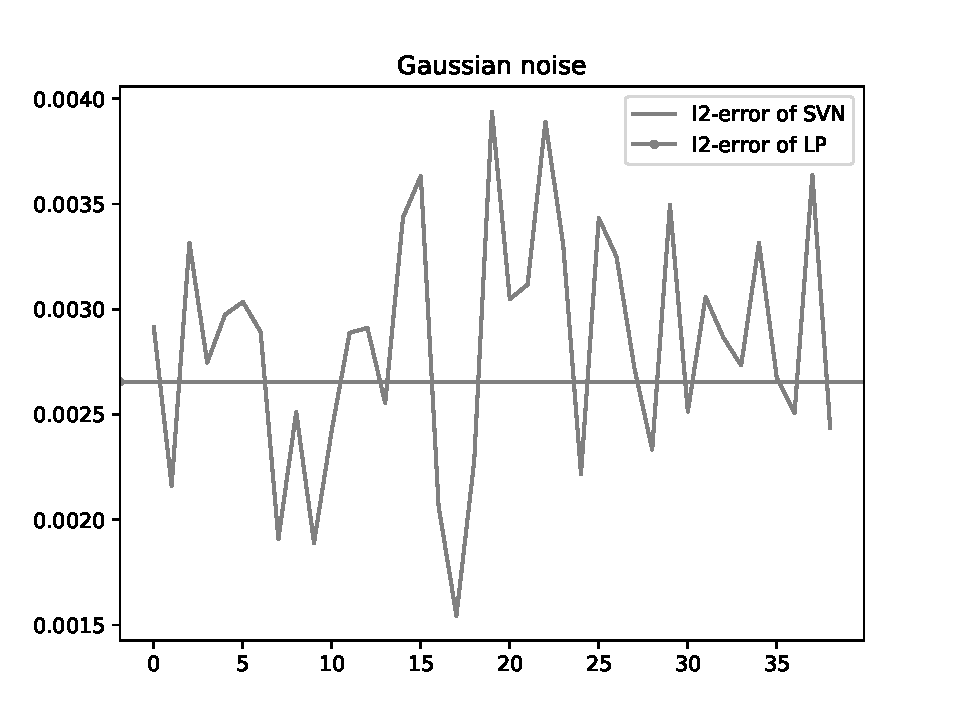
\includegraphics[width=4.9cm]{pics/chapter2/gaussian-svn.pdf}
    \captionof{figure}{}
    \end{subfigure}
    \begin{subfigure}[t]{0.3\textwidth}\label{svn-demo2}
    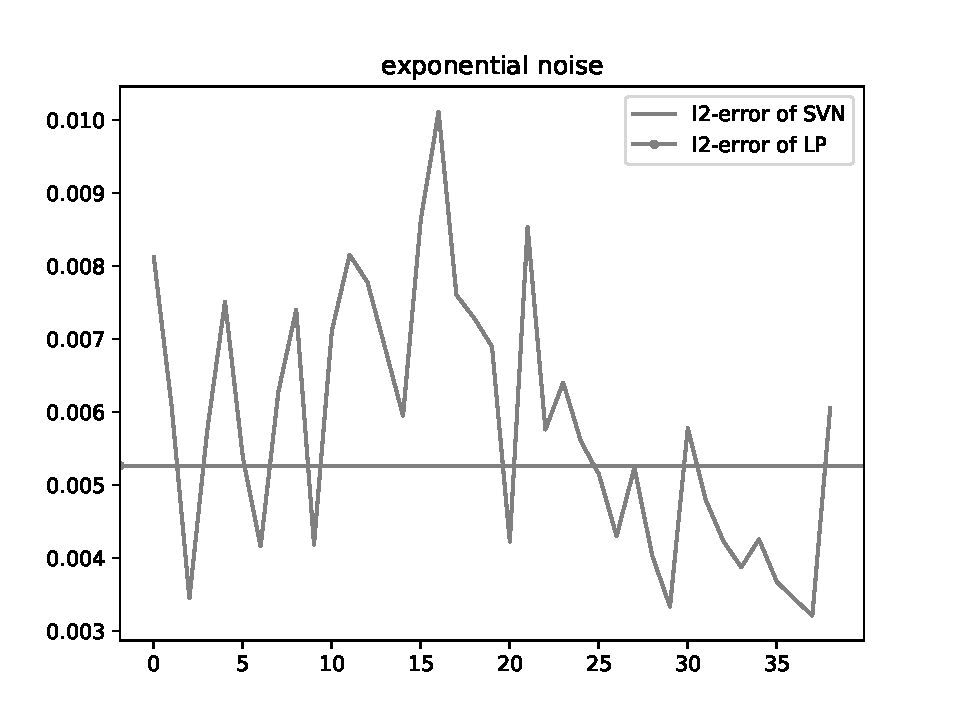
\includegraphics[width=4.9cm]{pics/chapter2/exp-svn.pdf}
    \captionof{figure}{}
    \end{subfigure}
    \begin{subfigure}[t]{0.3\textwidth}\label{svn-demo3}
    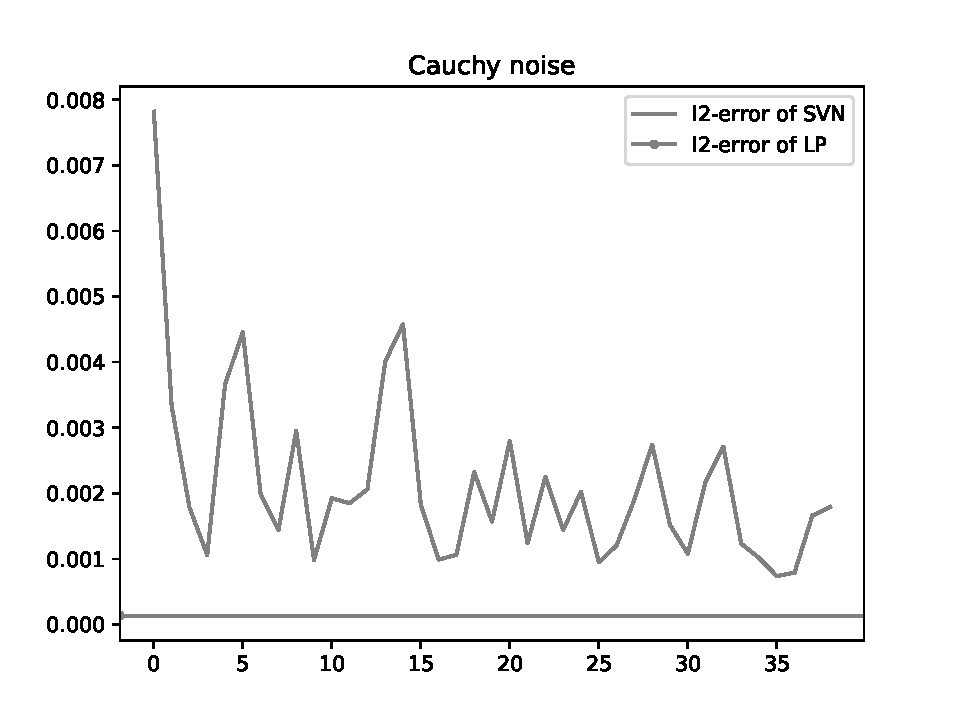
\includegraphics[width=4.9cm]{pics/chapter2/cauchy-svn.pdf}
    \captionof{figure}{}
    \end{subfigure}
    \caption{ \small SVN算法在各种噪声下的表现}
    \label{svn-noise}
\end{figure}

主要到算法3.2中我们使用最小绝对值回归估计量作为初始估计。在柯西噪声下,我们考虑了
最小二乘估计量作为初始估计的情况,来观察SVN算法的准确性。

\begin{figure}[H]
    \centering
    \begin{subfigure}[t]{0.3\textwidth}\label{svn-demo2}
    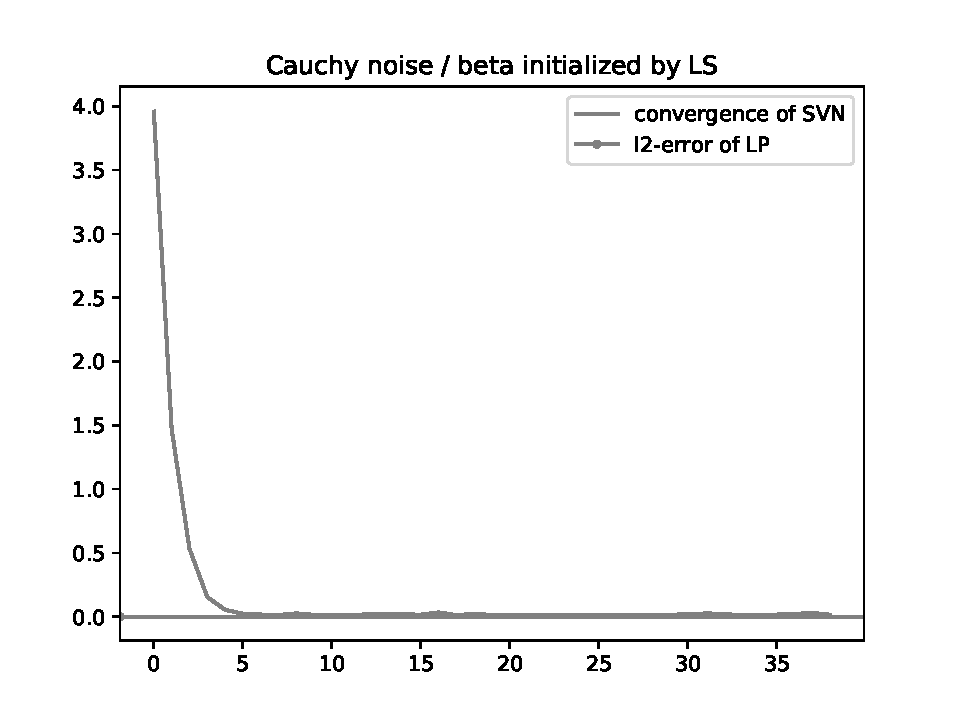
\includegraphics[width=4.9cm]{pics/chapter2/l2-svn-demo.pdf}
    \captionof{figure}{}
    \end{subfigure}
    \begin{subfigure}[t]{0.3\textwidth}\label{svn-demo3}
    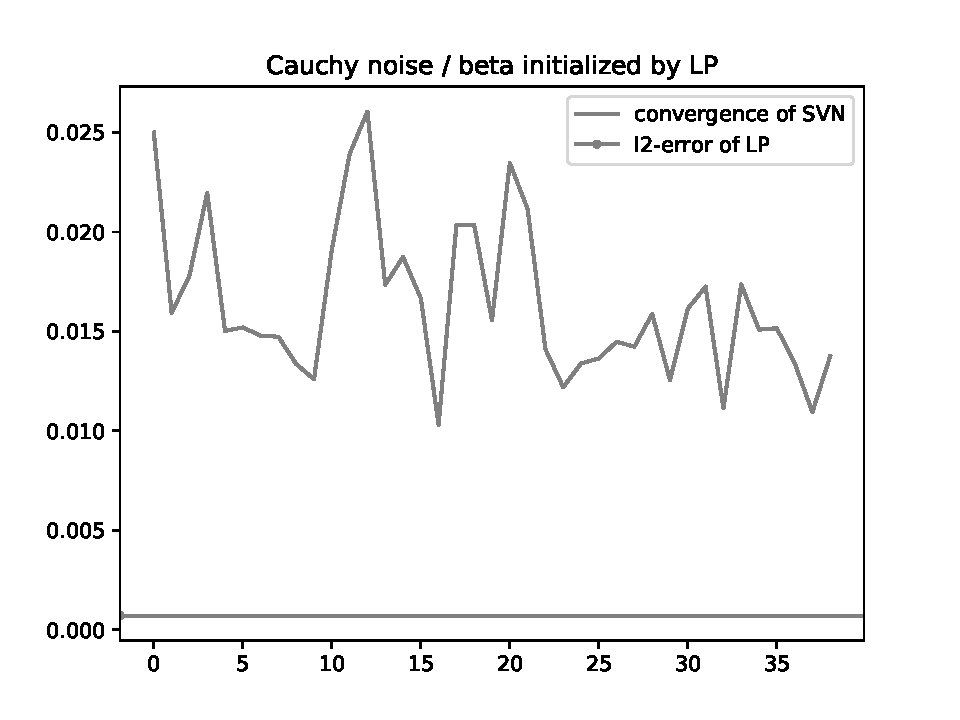
\includegraphics[width=4.9cm]{pics/chapter2/l1-svn-demo.pdf}
    \captionof{figure}{}
    \end{subfigure}
    \caption{ \small 最小二乘估计初始化}
    \label{svn-l2-demo}
\end{figure}

图\ref{svn-l2-demo}中横轴代表示迭代次数,纵轴代表示估计的误差平方和。实验结果表明,
选择最小二乘估计量作为初始值,SVN算法依然能够很快收敛。这启发我们
在使用最小绝对值回归时,如果最小二乘估计量是相合的,那么也可以通过最小二乘估计量产生初始估计,
这样一来,在计算中可做到完全避免直接求解最小绝对值回归问题。

需要说明的是,SVN算法的收敛速度和带宽选择有很大关系。
在选择了足够小的带宽时,SVN算法可快速收敛。图\ref{svn-demo}展示了SVN算法的收敛情况,
其中横轴代表示迭代次数,纵轴代表示相邻两次$\bm{\beta}$估计之差的平方和。
观察到SVN算法在带宽较小时收敛速度表现较好,这也符合该算法提出的理论基础。
在带宽选择较小($s$较小)时,SVN算法能够迅速收敛。
当然,如果我们选择了很大的带宽那么算法不能收敛。
\begin{figure}[H]
    \centering
    \begin{subfigure}[t]{0.3\textwidth}\label{svn-demo1}
    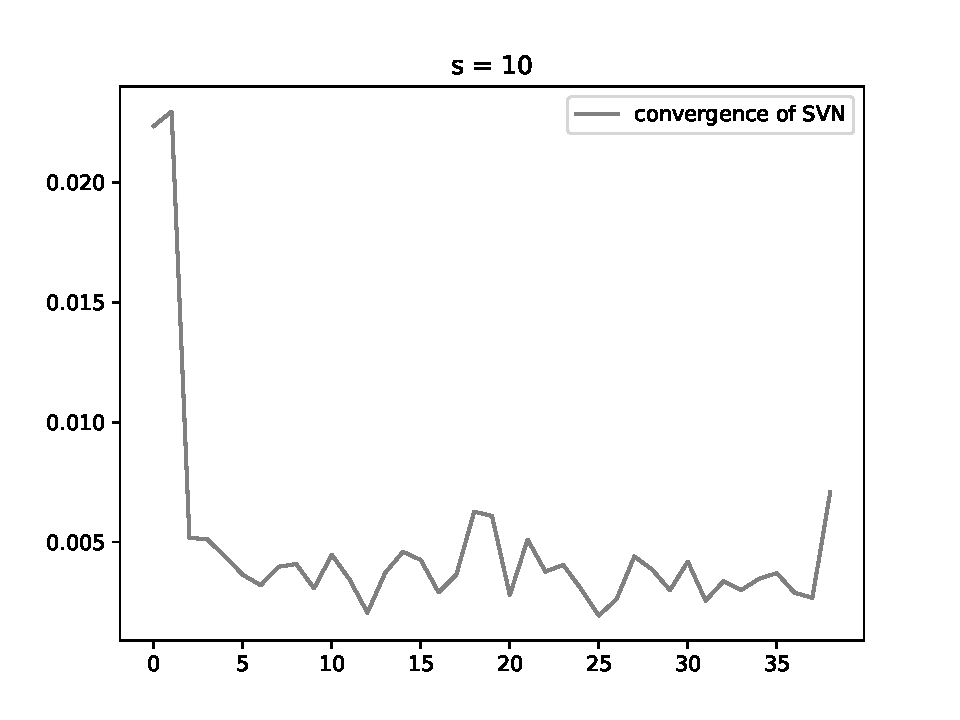
\includegraphics[width=4.9cm]{pics/chapter2/svn-con-1.pdf}
    \captionof{figure}{}
    \end{subfigure}
    \begin{subfigure}[t]{0.3\textwidth}\label{svn-demo2}
    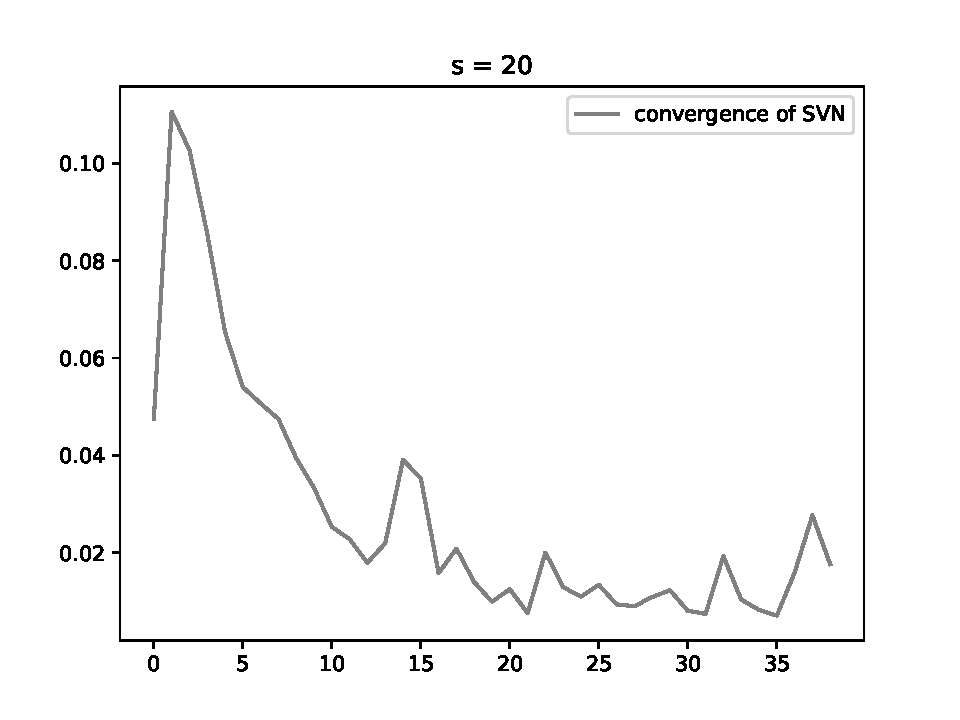
\includegraphics[width=4.9cm]{pics/chapter2/svn-con-2.pdf}
    \captionof{figure}{}
    \end{subfigure}
    \begin{subfigure}[t]{0.3\textwidth}\label{svn-demo3}
    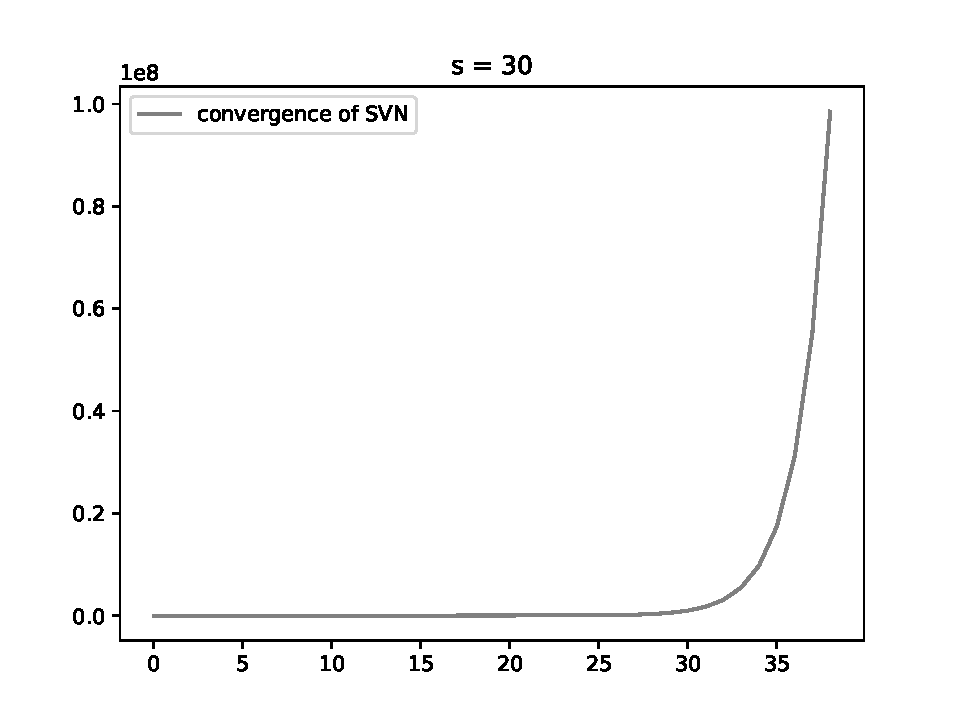
\includegraphics[width=4.9cm]{pics/chapter2/svn-con-3.pdf}
    \captionof{figure}{}
    \end{subfigure}
    \caption{ \small SVN算法的收敛情况}
    \label{svn-demo}
\end{figure}

然而在核密度估计中,一个更大的带宽意味着对该点密度估计包含了更多的样本信息,
选择过很小的带宽,可能造成对核密度估计不准,在应用中需要进行合理选择。

下面我们采用最小二乘估计进行初始化,并且设置终止条件为连续两次迭代后$\hat{\bm{\beta}}$的夹角小于某一常数阈值,
然后对算法的性能作进一步的比较。
这次我们将噪声设为正态噪声,但将其中10\%的数据添加柯西噪声,部分性能对比结果见表\ref{perfomance2}。

% Please add the following required packages to your document preamble:
% \usepackage{booktabs}
\begin{table}[H]
    \small
    \caption{部分性能结果对比}\label{perfomance2}
    \resizebox{\textwidth}{!}{
    \begin{tabular}{@{}ccccccccccc@{}}
        \toprule
        s & n     & p   & $\tau$ & Time(SVN) & Time(SVN-full) & Time(LP) & Time(AID) & $l_2$-error(SVN) & $l_2$-error(LS) & $l_2$-error(LP) \\ \midrule
        5 & 20000 & 10  & 12        & 0.12      & 0.42           & 0.17     & 2         & 0.0023        & 0.7304       & 0.0024       \\
        5 & 20000 & 50  & 8         & 1         & 7              & 3        & 13        & 0.0039        & 3.1548       & 0.0020       \\
        5 & 20000 & 100 & 14        & 10        & 28             & 19       & 41        & 0.0059        & 15.0373      & 0.0033       \\
        5 & 20000 & 200 & 27        & 81        & 130            & 170      & 124       & 0.0188        & 151.4039     & 0.0028       \\ 
        5 & 20000 & 500 & 40        & 437        & 437             & 1119       & 698        & 0.0259        & 245.0070      & 0.0026       \\
        \bottomrule
        \end{tabular}
    }
\end{table}

表\ref{perfomance2}中比较了设置终止条件的SVN算法、线性规划、不设置终止条件的SVN算法以及AID算法的计算时间(分别是Time(SVN)、Time(LP)、Time(SVN-full)
、Time(AID))。可以看出,SVN算法在计算效率上有明显的优势;同时表中记录了解和真实值差的$L_2$范数($l_2$-errors)。观察发现,
在柯西噪声数据下,SVN算法比最小二乘估计有小得多的估计误差,意味着它具有很好的稳健性。


\subsubsection{结论}
AID算法和SVN算法都可以用来求解最小绝对值回归,并且两者在数据规模较大的情况下,都明显快于线性规划。
SVN算法虽然不能保证取得最优解,但是它可以完全避免线性规划计算,因此在计算性能上很有优势;而AID算法
在小规模数据下不具有性能优势,然而在数据集很大时优势明显,并且AID算法最终的解就是对全部数据求解线性规划的结果,
因此它具有更好的稳健性。

我们的结论是,在数据能够服从线性模型时,对最小绝对值回归的计算推荐使用SVN算法,该算法具有很快的速度。
而在一般求解具有$min\ \Sigma_{i=1}^{n} |y_i - \bm{X}_i^T\bm{\beta}|$形式,但是数据能否服从线性模型未知时,
可以先使用最小二乘法拟合,并对模型做出检验然后进行算法选择。对于必须用线性规划来求解的形式类似问题,那么
建议使用AID算法来进行优化。

我们没有进行实验对比带有惩罚项的情况,原因在于:惩罚项主要用来对线性模型中用于系数稀疏化处理,
避免直接拟合的模型具有共线性,在实际应用中普遍使用$L_1$惩罚项。
我们通常已经假定了数据服从线性模型,所以此时SVN算法适用。并且前面提到LASSO算法具有很高的性能,而增加额外约束的线性规划
在速度上就更不具有优势,所以对于带有$L_1$惩罚项的最小绝对值回归,我们始终推荐使用SVN算法。


% \subsection{SVN-AID算法}
% 我们已经研究了AID和SVN两种方法,注意到AID算法的基础思想是具有普适性的。我们不妨再次分析使用AID算法
% 解决最小绝对值回归问题的实质:为了避免在整个数据集上一次性求解,我们使用聚类的方法,希望通过尽可能少的
% 计算来利用样本的信息。不妨将前文提到的AID算法称为AID-LP算法,它成功减少了解决最小绝对值回归问题的LP计算规模。

% 在AID算法求解最小绝对值回归时,
% 假设在第$t$次迭代中我们得到了$\bm{\beta}^{(t)}$,然后根据$\bm{\beta}^{(t)}$对现有的聚类进行拆解。
% 在下一步,我们重新计算该问题,直到达到问题最优解。而$\bm{\beta}^{(t)}$此时已经成功分离了许多聚类,
% 而这些聚类在下一个步骤中仍然全部需要进入计算,因为上一步的参数信息$\bm{\beta}^{(t)}$在下一步计算时被舍弃了。

% 而SVN算法,正是通过利用上一步的参数信息来构造代理变量简化计算。我们不妨结合两种算法的优点,将SVN算法
% 和AID算法结合起来,进一步优化对最小绝对值回归问题的求解。

% \begin{figure}[H]
%     \centering
%     \begin{subfigure}[t]{0.4\textwidth}\label{impro-demo1}
%     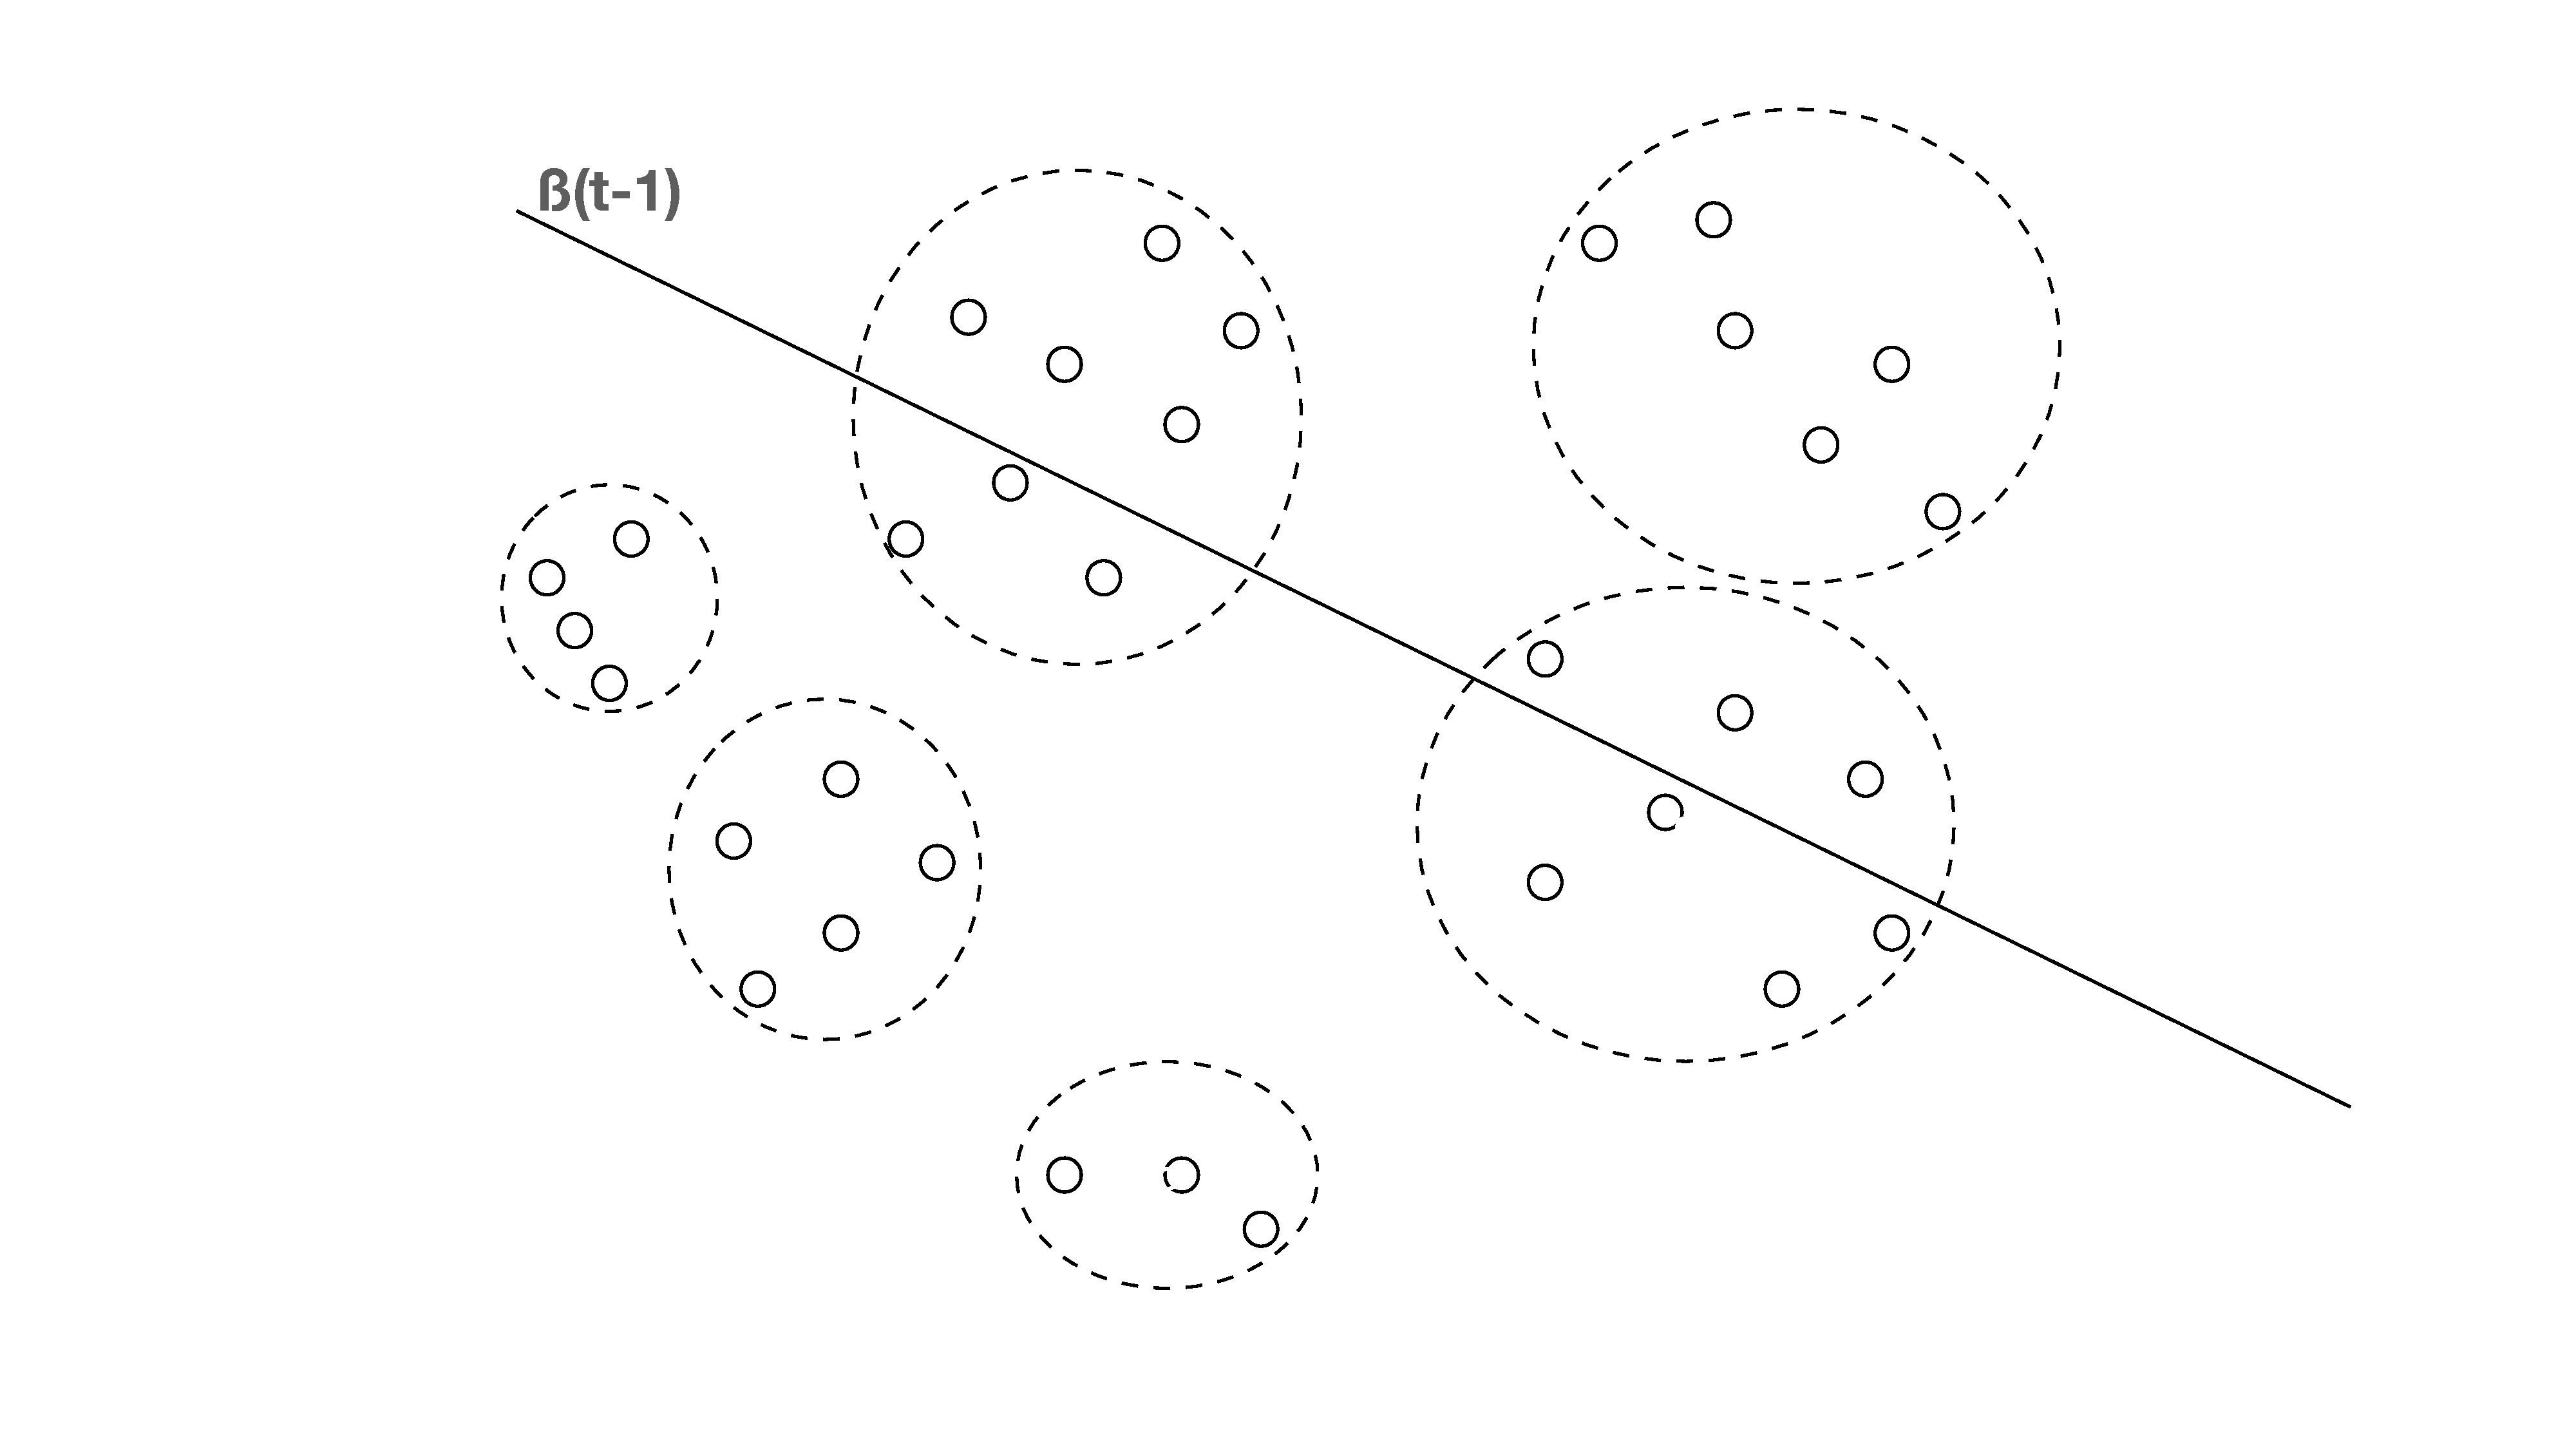
\includegraphics[width=8cm]{pics/chapter2/impro-demo-1.pdf}
%     \captionof{figure}{}
%     \end{subfigure}
%     \centering
%     \begin{subfigure}[t]{0.4\textwidth}\label{impro-demo2}
%     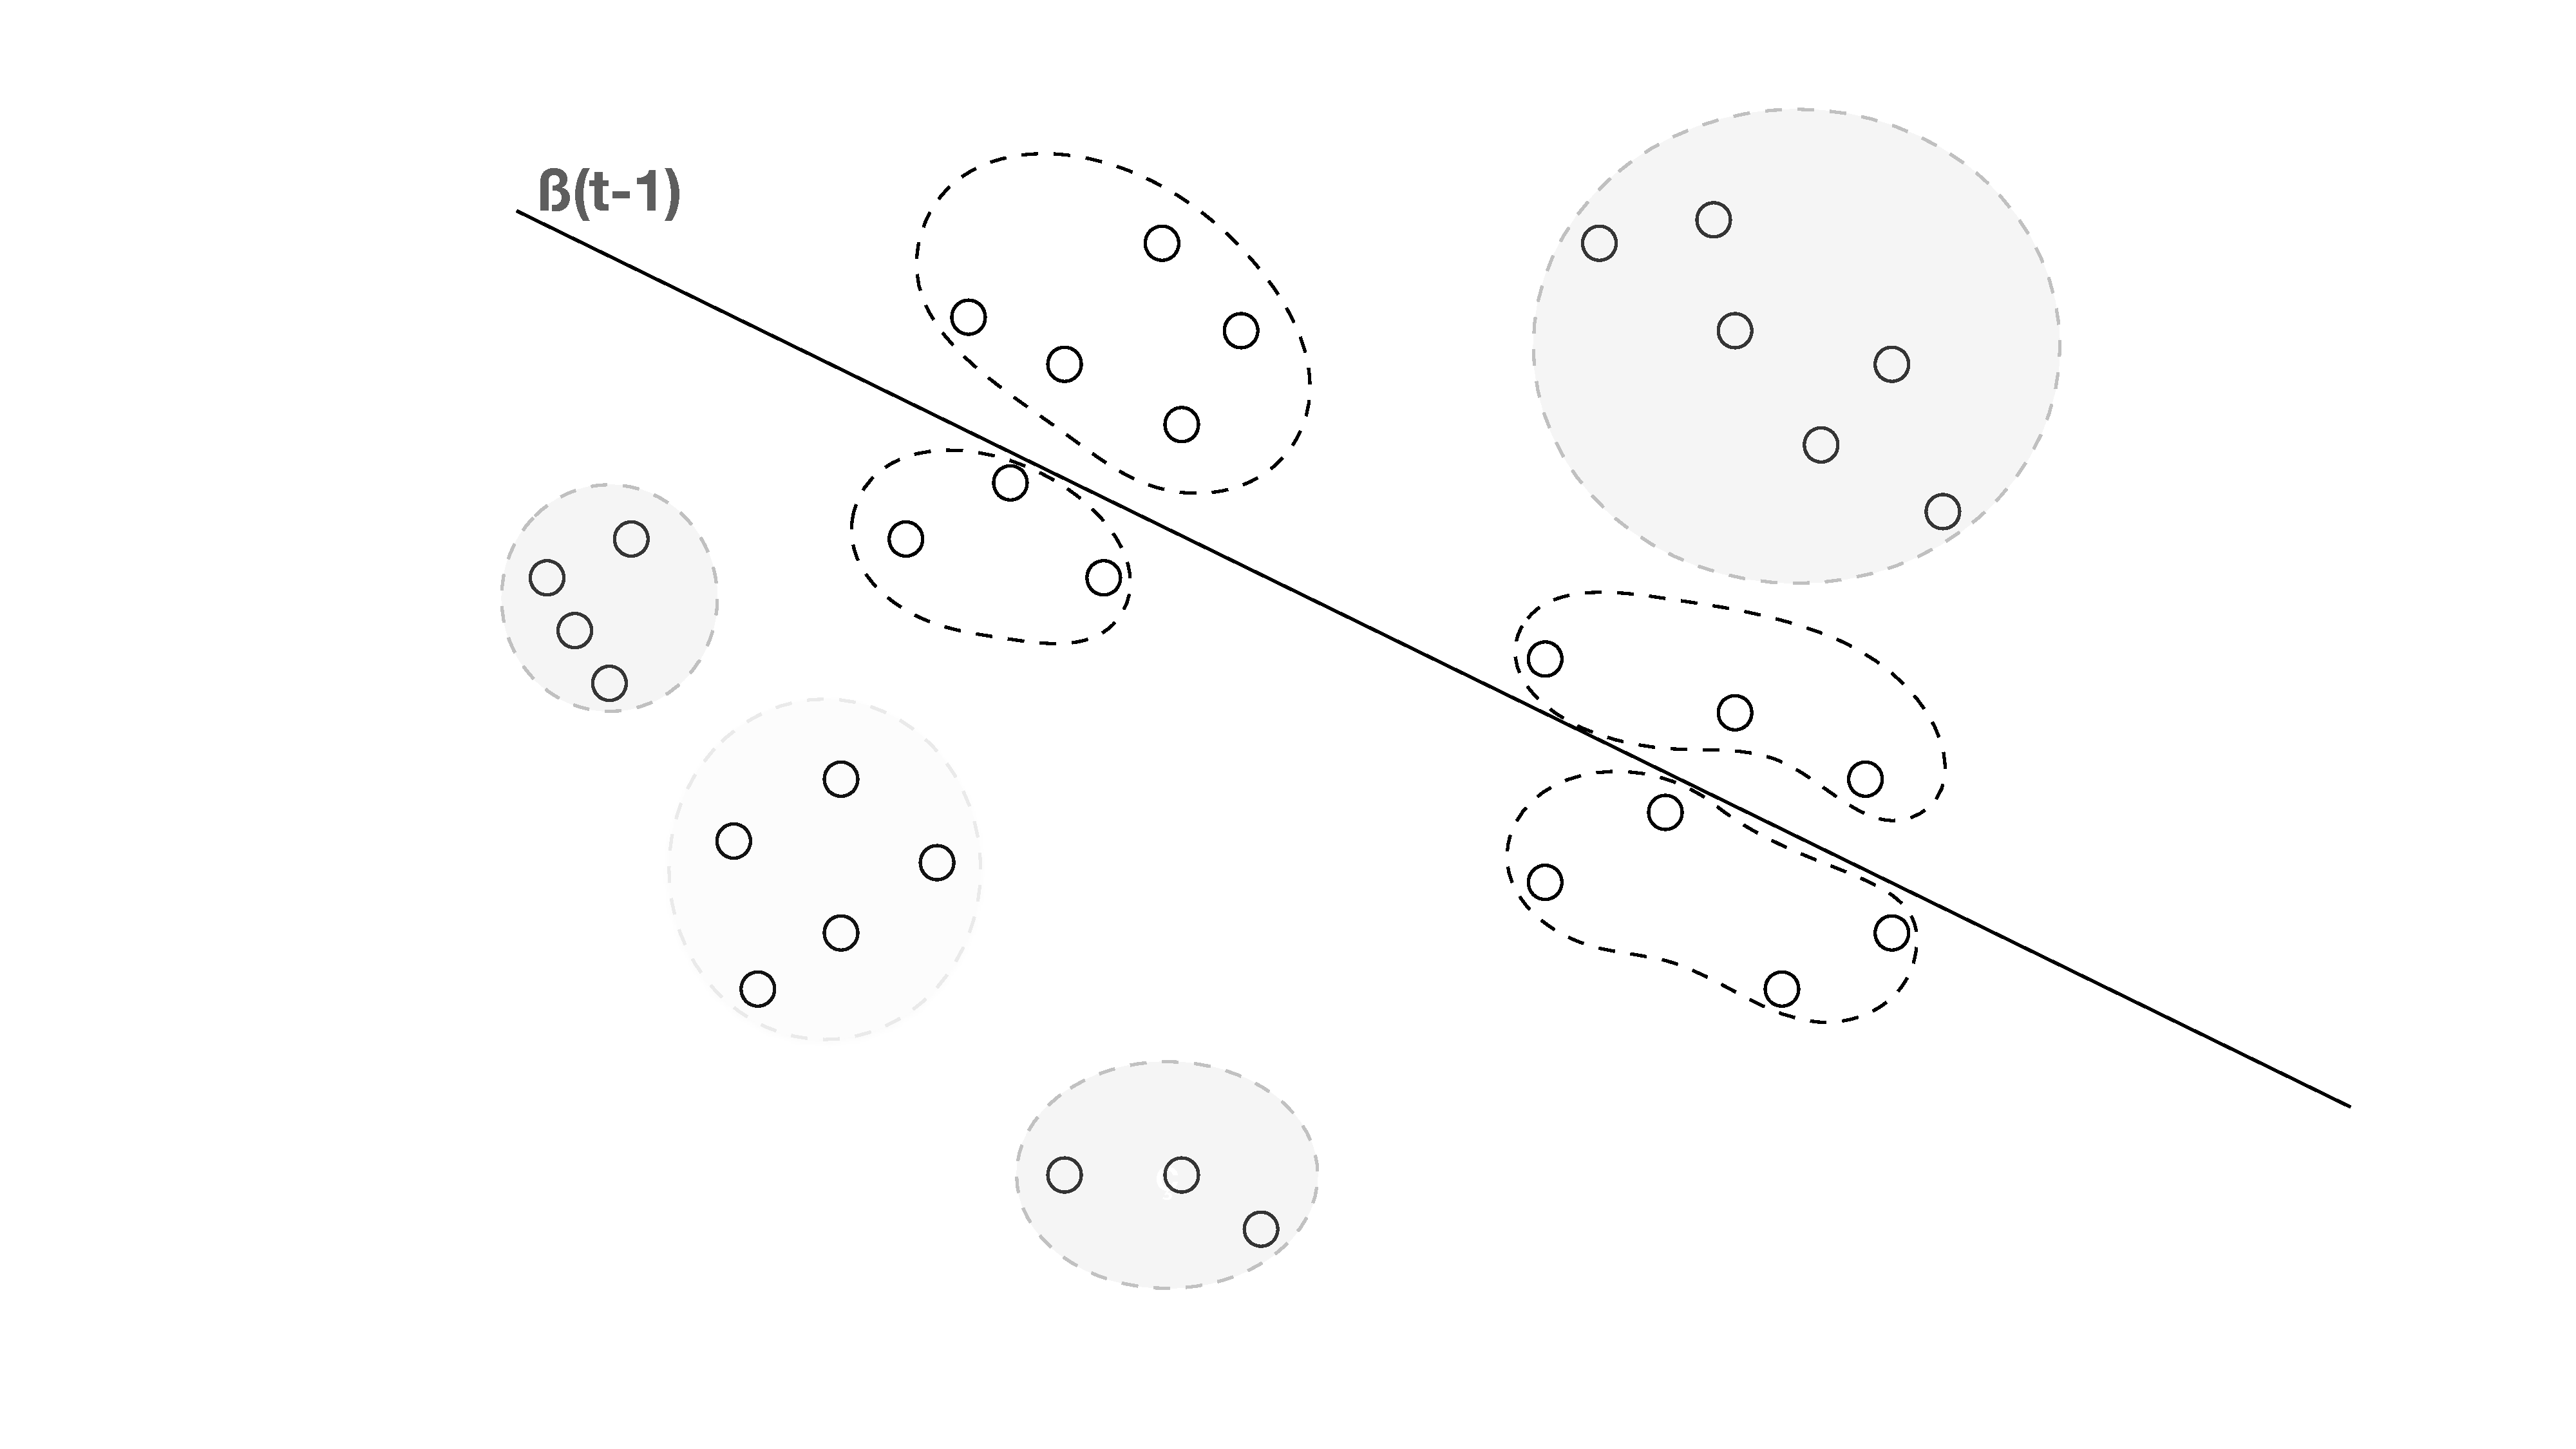
\includegraphics[width=8cm]{pics/chapter2/impro-demo-2.pdf}
%     \captionof{figure}{}
%     \end{subfigure}
%     \caption{ \small SVN-AID算法示意图}
%     \label{impro-demo}
% \end{figure}

% \subsubsection{算法步骤}
% 以下我们给出SVN-AID的步骤:
% 1)初始化:随机采样,进行最小绝对值回归,该步骤使用LP,得到$\hat{\bm{\beta}}^0$。根据各个样本点对该模型的拟合残差进行聚类。
% 2)记上一次迭代得出的系数估计为$\hat{\bm{\beta}}^t$,对当前聚类按照规则拆解。本步骤返回被拆解的聚类组成的集合,
% 舍弃上一步正确分类的聚类。
% 3)根据上一步返回的聚类集合,构造新数据集,并且按照\eqref{svny}构造代理变量数据集,并由\eqref{yl2loss}得出本轮估计。

% 具体见算法3.3,该算法通过舍弃正确分类的聚类,不断缩小问题规模,迭代优化上一步得出的参数估计值来进行对最优解的近似,
% 该算法在理论上可以极大减小AID算法的计算量,并且在舍弃大量样本点的同时,充分利用了前面步骤得出的参数信息。

% \begin{table}[H]%%%%%%开始表格
%     \centering%把表居中
%     \begin{tabular}{{p{0.9\columnwidth}}}%三个c代表该表一共三列,内容全部居中
%     \toprule%第一道横线 表头
%     {\heiti 算法}{\bf 3.3} SVN-AID算法\\
%     \midrule%第二道横线 符号+解释+单位 中间用&隔开
%     输入:$Y$和$\bm{X}$的样本$\bm{Y} = (Y_1, Y_2, ..., Y_n)$,$\bm{X} = (\bm{X}^T_1, \bm{X}^T_2, ..., \bm{X}^T_n)$,
%     迭代次数$\tau$,核函数$K$,依赖于迭代次数的带宽$h^{(t)}$,$(t = 1, ..., \tau)$。
%     \\
%     初始化:给出初始估计,$\hat{\bm{\beta}}^{(0)} $,对每一个样本点$(X_i, Y_i)$根据$Y_i - X_i^T\bm{\beta} $的结果进行
%     K-means聚类,得到聚类结果$C^{(0)} = \{C_1^{(0)}, C_2^{(0)}, ... , C_K^{(0)}\}$。
%     \\
%     对于$t = 1, ..., \tau$:\\
%         1)根据上一轮$\hat{\bm{\beta}}^{(t-1)}$,计算带宽$h^{(t)}$和
%         $\hat{f(0)}^{(t)} = \frac{1}{K^{(t)}h^{(t)}}\sum_{i=1}^{K^{(t)}}K(Y_i - \bm{X}_i^T\hat{\bm{\beta}}^{(t-1)})$。\\
%         据\eqref{svny}在当前聚类上构造替代变量$\tilde{Y} = (\tilde{Y}_1, ..., \tilde{Y}_{K^{(t)}})$;
%         求解
%         $$
%             \hat{\bm{\beta}}^{(t)} = \underset{\bm{\beta} \in \mathbb{R}^{p}}{\operatorname{arg\ min}}
%             \frac1{K^{(t)}} \sum_{k=1}^{K^{(t)}}|C_i^{(t)}|(\tilde{Y}_k - \bm{X}_k^T\bm{\beta})^2
%         $$
%         2)对于$k = 1, ..., K^{(t)}$,计算$\theta_i = y_i - \sum_{j \in J}x_{ij}\hat{\bm{\beta}}_j^{(t)}$,
%         根据$\theta_i$符号异同,将$C^{(t)}_k$分成两个集合,$C_{k+}^{(t)} = \{i \in C_k^{(t)} | \theta_i > 0\}$ ,
%         $C_{k-}^{(t)} = \{i \in C_k^{(t)} | \theta_i < 0\}$,这两个集合在下一步形成新的聚类,
%         即$C^{(t+1)} \leftarrow C^{(t+1)}\bigcup \{ C_{k+}^{(t)}, C_{k-}^{(t)}\}$。 
        
%         输出:$\bm{\beta}^{(\tau)}$
%     \\
%     \bottomrule%第三道横线
%     \end{tabular}
% \end{table}%%%%%%结束表格

% \subsubsection{数值模拟实验}

\subsection{本章小结}

本章首先简要介绍了$L_1$范数的概念,列举了一些其在经济数据分析领域的应用。随后,讨论了
最小绝对值回归的稳健性和其求解方法。

最小绝对值回归已经广泛应用在高维宏观经济数据的处理中,但是它在应用中存在一定的性能问题。
本章介绍了两种可以应用于最小绝对值回归的优化手段:聚类——迭代拆解算法和基于替代变量的估计方法。
进行了数值模拟实验,分析了其优缺点,并给出了其在实际应用中的几点建议。

聚类——迭代拆解算法
是一种非常好的思想,它结合了机器学习中聚类的方法,聚类的作用可以将信息进行提纯,在经过处理
后的数据集上解决原始问题对应的加权优化问题,可以避免直接解决原始问题而耗费庞大的计算量。
聚类——迭代拆解算法可以应用于解决最小绝对值回归问题,它在一定程度上减少了线性规划的计算量,
并且在理论上具有最优解,即它的解一定可以和直接对所有数据求解进行线性规划问题一样好。

另外,本章介绍了另外一种巧妙的算法——一种基于替代变量的迭代算法,该算法通过
构造替代变量,从而将原来需要通过线性规划解决的最小绝对值回归问题转化为
解决替代变量的最小二乘问题。这样一来,计算的复杂度就大大降低。该方法在
实际应用中性能表现十分优秀,但是需要注意带宽的选择。

聚类——迭代拆解算法对和最小绝对值回归目标函数相同的任何优化问题均适用;
然而SVN算法在其理论基础上需要假设线性模型成立,需要结合我们面临的实际问题酌情使用。

最后,我们在本章对最小绝对值回归性能优化的研究,会对后续
章节中优化$L_1$范数主成分分析法估计近似因子模型的求解算法有推动作用。
